\documentclass[a4paper, 7pt, landscape]{scrartcl}
\usepackage[german]{babel}
\usepackage[utf8]{inputenc}
\usepackage{multicol}
\usepackage{geometry}
\usepackage{graphicx}
\usepackage{wrapfig}
\usepackage{enumitem}
\usepackage{fancyhdr}
\usepackage{index}
\usepackage{sectsty}
\usepackage{mwe}
\usepackage{comment}
\usepackage{lipsum}
\usepackage{titlesec}
\usepackage[dvipsnames]{xcolor}
\usepackage{amsmath}
\usepackage{amssymb}
\usepackage{listings}

%Define Math Commands:
\newcommand*{\field}[1]{\mathbb{#1}}%
\newcommand{\Mod}[1]{\ (\mathrm{mod}\ #1)}

%Image Folder:
\graphicspath{{../img/}}

%format
\geometry{top=0.4cm,left=0.5cm,right=0.5cm,bottom=0.4cm}
\setlist{topsep=0pt, leftmargin=5mm, nolistsep}

% Code Snippets

\definecolor{javared}{rgb}{0.6,0,0} % for strings

\lstset{
language=java,
basicstyle=\fontsize{7}{7} \ttfamily,
keywordstyle=\bfseries\color{RoyalBlue},
stringstyle=\color{javared},
commentstyle=\color{MidnightBlue},
morecomment=[s][\color{MidnightBlue}]{/**}{*/},
tabsize=2,
showspaces=false,
showstringspaces=false,
texcl = true,
rulecolor = \color{black},
breaklines = true,
aboveskip = 0.5em,
belowskip = 0.5em
}




% Define Section Format
\titleformat{name=\section}[block]
{\sffamily\normalsize}
{}
{0pt}
{\colorsection}
\titlespacing*{\section}{0pt}{0pt}{0pt}

\newcommand{\colorsection}[1]{%
\colorbox{MidnightBlue!40}{\parbox{0.98\linewidth}{\color{black}\thesection\ #1}}}


% Define Subsection Format
\titleformat{name=\subsection}[block]
{\sffamily\small}
{}
{0pt}
{\colorsubsection}
\titlespacing*{\subsection}{0pt}{0pt}{0pt}

\newcommand{\colorsubsection}[1]{%
\colorbox{YellowGreen!50}{\parbox{0.98\linewidth}{\color{black}\thesubsection\ #1}}}

% Define SubSubsection Format
\titleformat{name=\subsubsection}[block]
{\sffamily\small}
{}
{0pt}
{\colorsubsubsection}
\titlespacing*{\subsubsection}{0pt}{0pt}{0pt}

\newcommand{\colorsubsubsection}[1]{%
\colorbox{Goldenrod!50}{\parbox{0.98\linewidth}{\color{black}\thesubsubsection\ #1}}}

% -----------------------------------------------------------------------
\begin{document}
    %	\pagecolor{p}
    %	\color{t}
    \setlength{\columnseprule}{0.4pt}
    \footnotesize
    \begin{multicols*}{3}

        %! Author = Philipp Emmenegger
%! Date = 30/06/2021

\section{Introduction}
\subsection{Pattern Definition}
\begin{itemize}
    \item Descriptions of successful engineering stories
    \item Address recurring problem
    \item Descripe generic solution that worked
    \item Tell about the forces of the problem (why is the problem hard)
    \item Tell about the engineering trade-offs  to take (Benefits / Liabilities)
    \item Solution (Implementation)
\end{itemize}

\subsection{Type of Patterns}
\begin{itemize}
    \item Architecture Patterns (Waiting Room)
    \item Software Patterns
    \begin{itemize}
        \item Design Pattern (Elements of Reusable Object-Oriented Sofware)
        \item Pattern-oriented Software Architecture (POSA)
    \end{itemize}
    \item Organizational Patterns
    \item Learning and Teaching Patterns
    \item Documentation Patterns
\end{itemize}

\subsection{Pattern Formats}
\subsubsection{POSA}
\begin{itemize}
    \item Pattern name
    \item Intent
    \item Problem
    \item Solution
    \item Benefits / Liabilities
\end{itemize}
\subsubsection{Fault Tolerance}
\begin{itemize}
    \item Name
    \item Intent
    \item Solution
    \item Benefits / Liabilities
\end{itemize}
\subsubsection{MAPI}
\begin{itemize}
    \item Name
    \item Intent
    \item Consequences
\end{itemize}
\subsubsection{Game Programming Patterns}
\begin{itemize}
    \item Name
    \item Problem
    \item Engineering Story that worked
    \item Benefits / Liabilities
    \item Solution
\end{itemize}

\subsection{What are Patterns not?}
\begin{itemize}
    \item Silver bullet
    \item Novices Tool
    \item Ready Made Components
    \item Means to turn off your brain
\end{itemize}

        \section{GoF Patterns}
\subsection{Observer}
Define a one-to-many dependency between objects so that when one object changes state, all its dependents are notified and updated automatically.\\
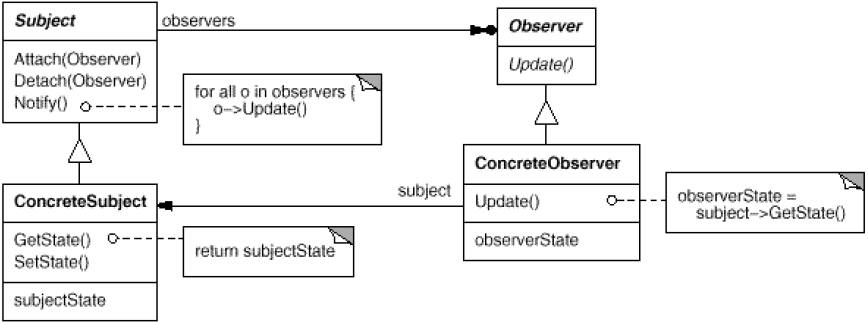
\includegraphics[width=\linewidth]{./img/observer.png}

\subsection{Strategy}
Define a family of algorithms, encapsulate each one, and make them interchangeable. Strategy lets the algorithm vary independently from clients that use it.\\
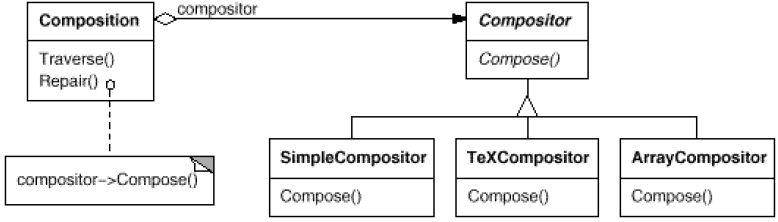
\includegraphics[width=\linewidth]{./img/strategy.png}

\subsection{Template Method}
Define the skeleton of an algorithm in an operation, deferring some steps to subclasses. Template Method lets subclasses redefine certain steps of an algorithm without changing the algorithm's structure.\\
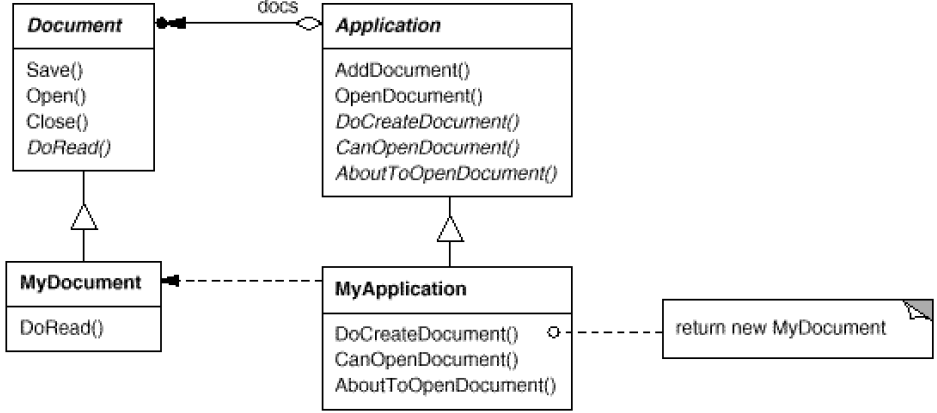
\includegraphics[width=\linewidth]{./img/template_method.png}

\subsection{Factory Method}
Define an interface for creating an object, but let the subclass decide which class to instantiate. Factory Method lets a class defer instantiation to subclasses.\\
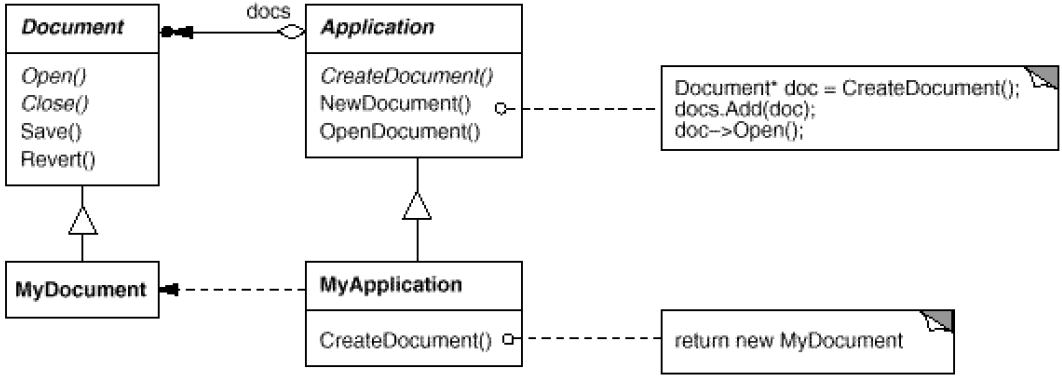
\includegraphics[width=\linewidth]{./img/factory_method.png}

\subsection{Abstract Factory}
Provide an interface for creating families of related or dependant objects without specifying their concrete classes.\\ 
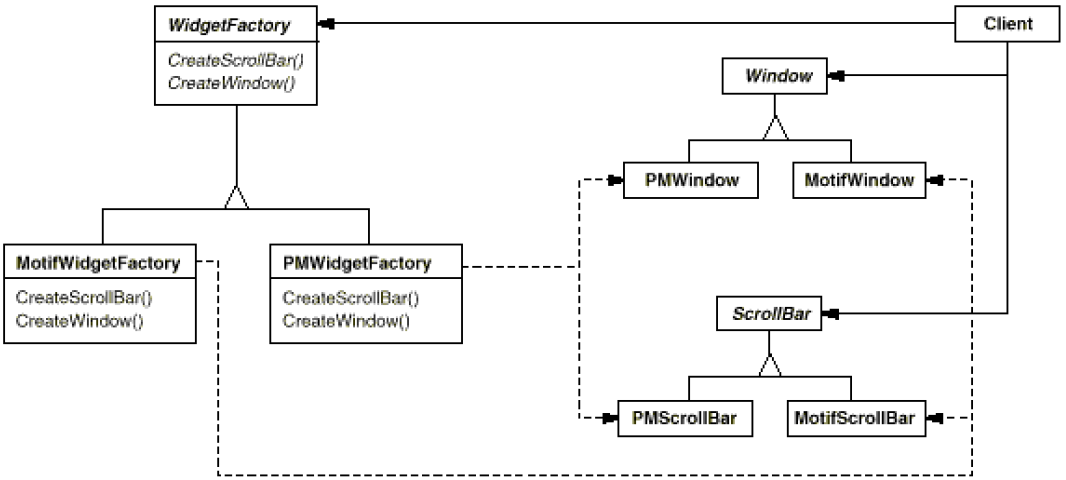
\includegraphics[width=\linewidth]{./img/abstract_factory.png}

\subsection{Prototype}
Specify the kinds of objects to create using a prototypical instance, and create new objects by copying this prototype.\\ 
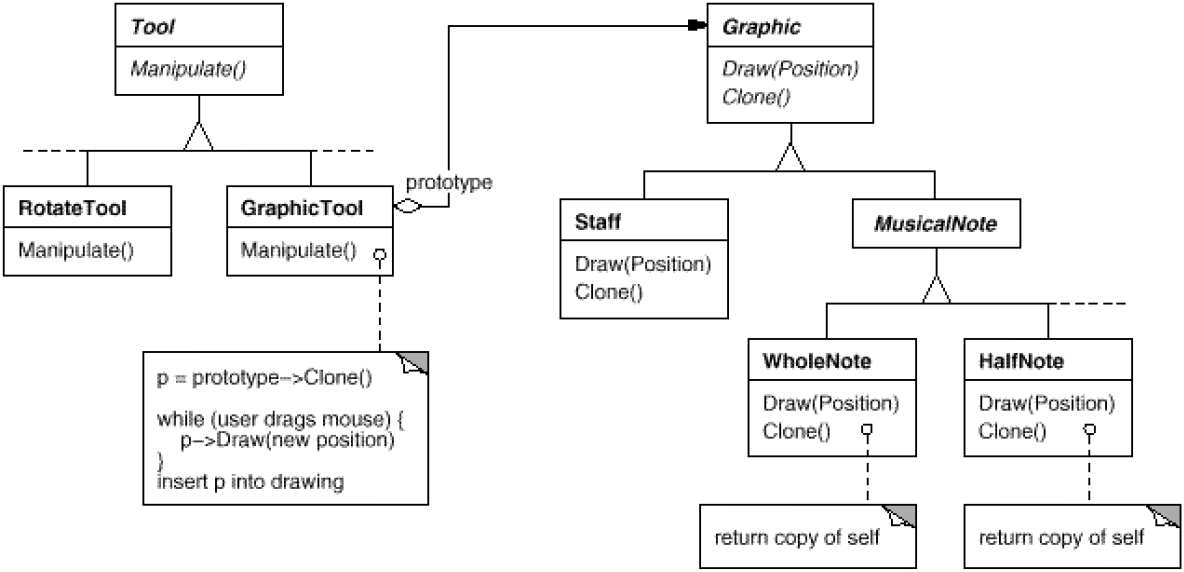
\includegraphics[width=\linewidth]{./img/prototype.png}

\subsection{Composite}
Compose objects into tree structures to represent part-whole hierarchies. Composite lets clients treat individual objects and compositions of objects uniformly.\\ 
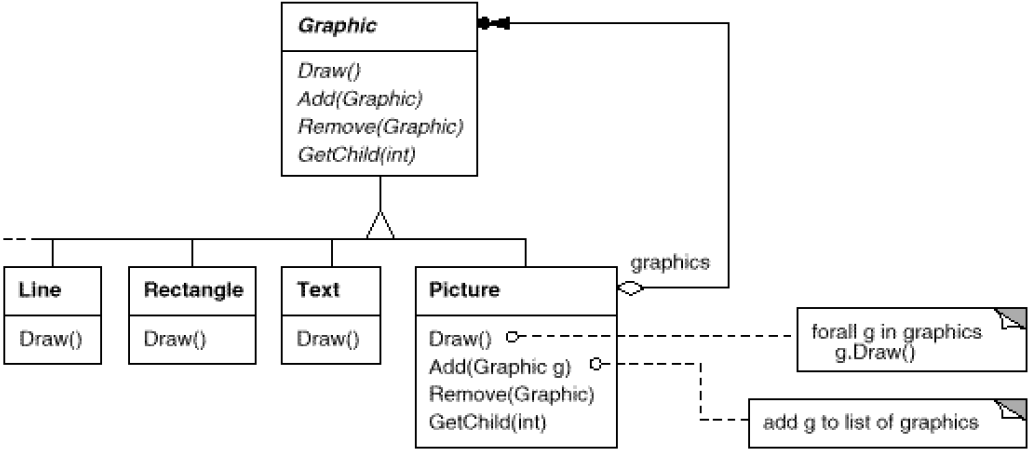
\includegraphics[width=\linewidth]{./img/composite.png}


\subsection{Decorator}
Attach additional responsibilities to an object dynamically. Decorators provide a flexible alternative to subclassing for extending functionality.\\ 
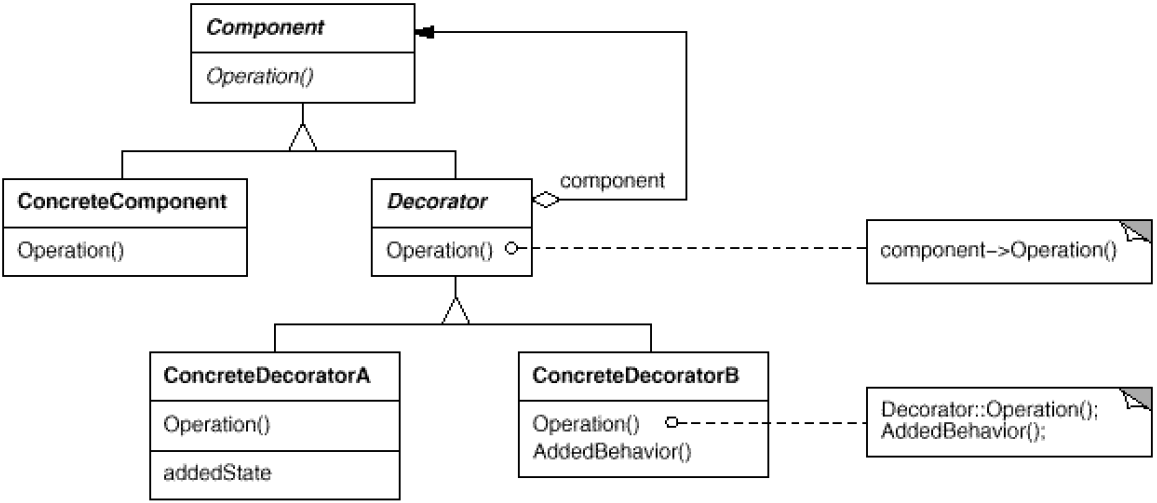
\includegraphics[width=\linewidth]{./img/decorator.png}

\subsection{Adapter}
Convert the interface of a class into another interface clients expect. Adapter lets classes work together that couldn't otherwise because of incompatible interfaces.\\ 
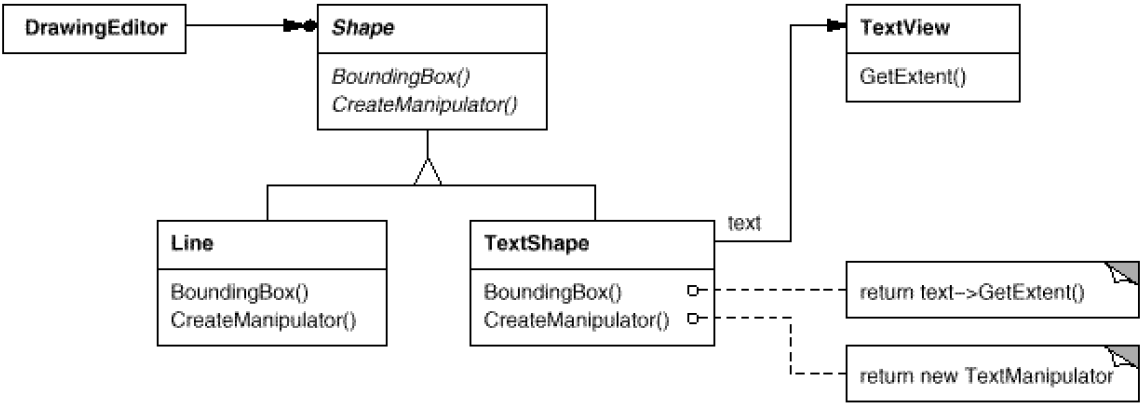
\includegraphics[width=\linewidth]{./img/adapter.png}

\subsection{Proxy}
Provide a surrogate or placeholder for another object to control access to it.\\ 
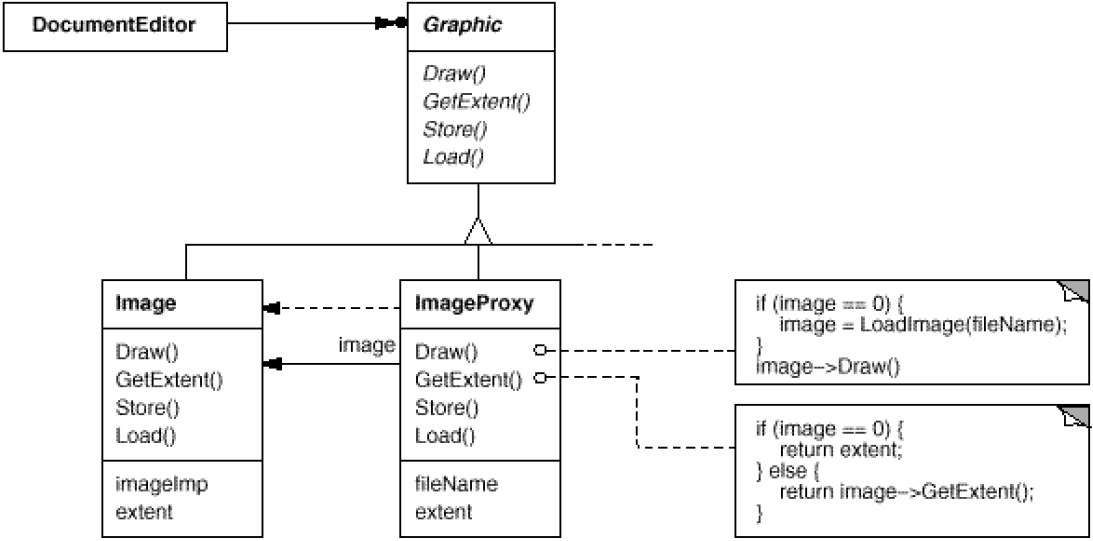
\includegraphics[width=\linewidth]{./img/proxy.png}

\subsection{Facade}
Provide a unified interface to a set of interfaces in a subsystem. Facade defines a higher-level interface that makes the subsystem easier to use.\\ 
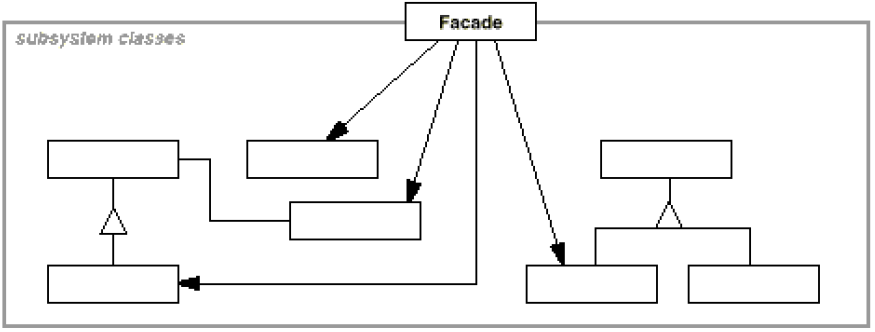
\includegraphics[width=\linewidth]{./img/facade.png}

\subsection{Mediator}
\subsubsection{Problem}
\begin{itemize}
    \item Object Structures may result in many connections between objects
    \item In the worst case, every object ends up knowing about every other
\end{itemize}
\textbf{Intent:}
\begin{itemize}
    \item How can strong coupling between multiple objects be avoided and communication simplified?
\end{itemize}
\subsubsection{Solution}
Define an object that encapsulates how a set of objects interact. Mediator promotes loose coupling by keeping objects from referring to each other explicitly, and lets you vary their interaction independently.\\ 
\textbf{Mediator:} Encapsulates how a set of objects interact\\ 
\textbf{Colleaues:} Refer to Mediator; this promotes loose coupling\\ 
\textbf{Static Structure:}\\
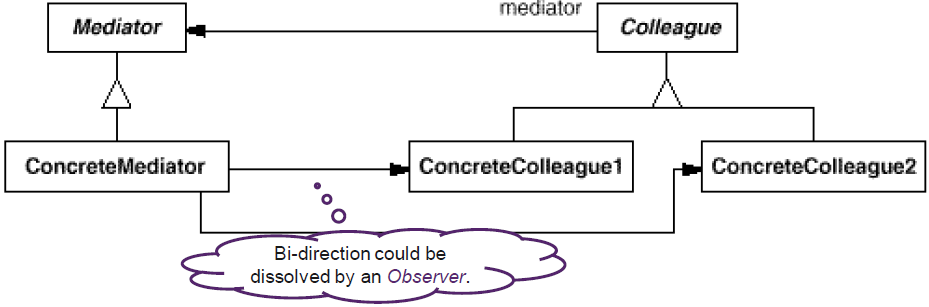
\includegraphics[width=\linewidth]{./img/mediator_static.png}
\textbf{Dynamics:}\\ 
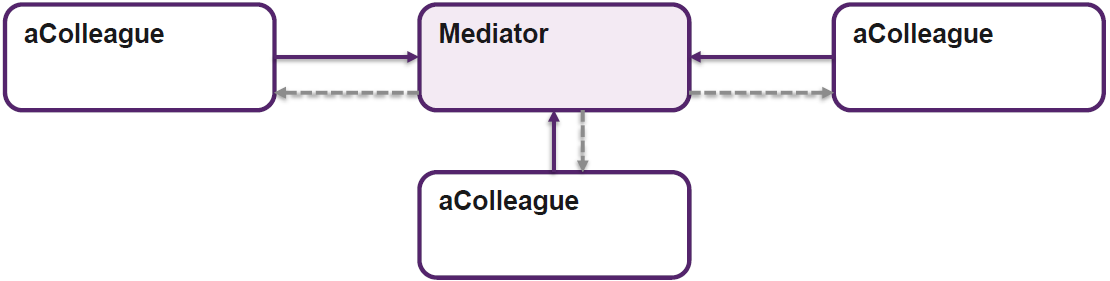
\includegraphics[width=\linewidth]{./img/mediator_dynamic.png}
\subsubsection{Implementation}
\begin{itemize}
    \item Mediator as an Observer
    \item Colleagues act as Subject
\end{itemize}
\textbf{Known Uses:}
\begin{itemize}
    \item Message Bus Systems
    \item Redux Dispatcher
\end{itemize}
\subsubsection{Summary}
\textbf{Benefits:}
\begin{itemize}
    \item Colleague classes may become more reusable, low coupling
    \item Centralizes control of communication between objects
    \item Encapsulates protocols
\end{itemize}
\textbf{Liabilities:}
\begin{itemize}
    \item Adds complexity
    \item Single point of failure
    \item Limits subclassing (of mediator class)
    \item May result in hard maintainable monoliths
\end{itemize}

\subsection{Memento}
\subsubsection{Problem}
\begin{itemize}
    \item Sometimes it's necessary to record the internal state of an object
    \item Objects normally encapsulate their state, making it inaccessible
\end{itemize}
\textbf{Intent:}
\begin{itemize}
    \item How can the state of an object be externalized without violating its encapsulation?
\end{itemize}
\subsubsection{Solution}
Without violating encapsulation, capture and externalize an objects internal state so that the object can be restored to this state later.\\
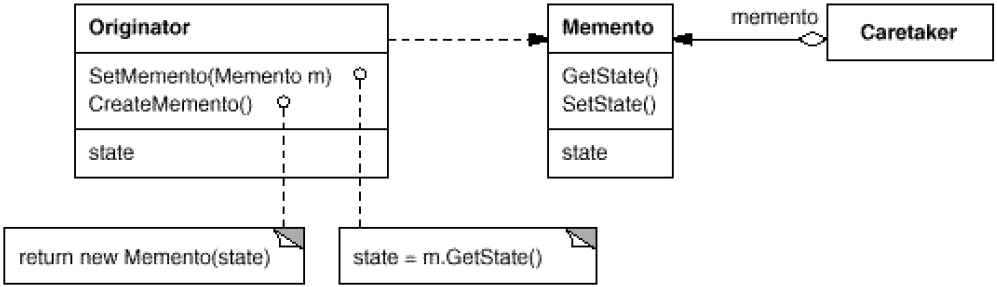
\includegraphics[width=\linewidth]{./img/memento.png}
\textbf{Dynamics:}\\ 
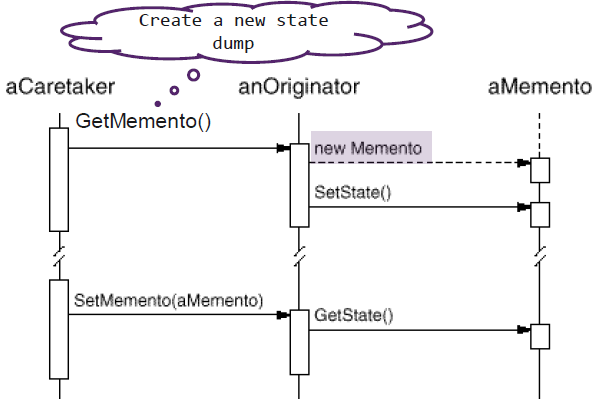
\includegraphics[width=0.7\linewidth]{./img/memento_dynamic.png}

\subsubsection{Participants}
\textbf{Memento}
\begin{itemize}
    \item Stores some / all the internal state of the Originator
    \item Allows only the originator to access its internal information
\end{itemize}
\textbf{Originator}
\begin{itemize}
    \item Can create Memento objects to store its internal state at strategic points
    \item Can restore own state to what the Memento object dictates
\end{itemize}
\textbf{Caretaker}
\begin{itemize}
    \item Stores the Memento objects
    \item Cannot explore / operate the contents 
\end{itemize}
\subsubsection{Implementation}
\begin{itemize}
    \item Originator creates memento and passes over its internal state
    \item Can be combined with Factory Method
    \item Declare Originator as \textit{friend} of Memento, so Originator can read out its properties
\end{itemize}
\subsubsection{Summary}
\textbf{Benefits}
\begin{itemize}
    \item Internal State of an object can be saved and restored at any time
    \item Encapsulation of attributes is not harmed
    \item State of objects can be restored later
\end{itemize}
\textbf{Liabilities}
\begin{itemize}
    \item Creates a complete copy of the object every time, no diffs (memory usage)
    \item No direct access to saved state, it must be restored first
\end{itemize}


\subsection{Command}
\subsubsection{Problem}
\begin{itemize}
    \item Decouple the decision of what to execute from the decision of when to execute
    \item The execution needs an additional parametrization context
\end{itemize}
\textbf{Intent:}
\begin{itemize}
    \item How can commands be encapsulated, so that they can be parameterized, scheduled, logged and/or undone?
\end{itemize}
\subsubsection{Solution}
Encapsulate a request as an object, thereby letting you parameterize clients with different requests, queue or log requests, and support undoable operation.\\ 
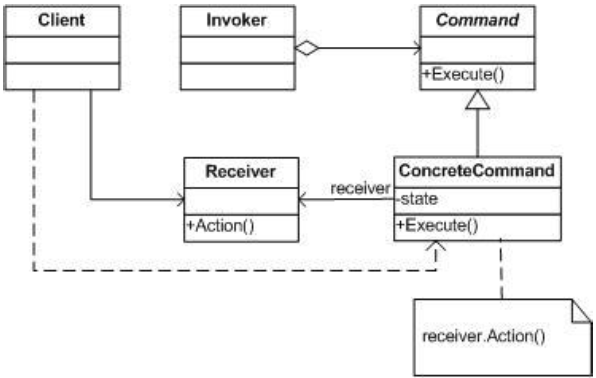
\includegraphics[width=\linewidth]{./img/command.png}
\textbf{Dynamics:}\\ 
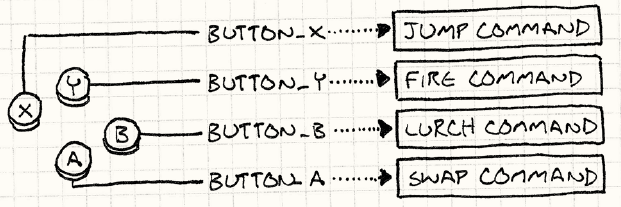
\includegraphics[width=\linewidth]{./img/command_dynamic.png}
\subsubsection{Summary}
\textbf{Benefits:}
\begin{itemize}
    \item The same command can be activated from different objects
    \item New commands can be introduced quickly and easily
    \item Command objects can be saved in a command history
    \item Provides inversion of control, encourages decoupling in both time and space
\end{itemize}
\textbf{Liabilities:}
\begin{itemize}
    \item Large designs with many commands can introduce many small command classes mauling the design
\end{itemize}

\subsection{Command Processor}
\subsubsection{Problem}
\begin{itemize}
    \item Common UI applications support do and multiple undo steps
    \item Steps forward and backward are accessible in a history
\end{itemize}
\textbf{Intent:}
\begin{itemize}
    \item How could we manage command objects, so the execution is seperated from the request and the execution can be undone later?
\end{itemize}
\subsubsection{Solution}
Separate the request for a service from its execution. A command processor component manages requests as separate objects, schedules their execution, and provides additional services such as the storing of request objects for later undo.\\ 
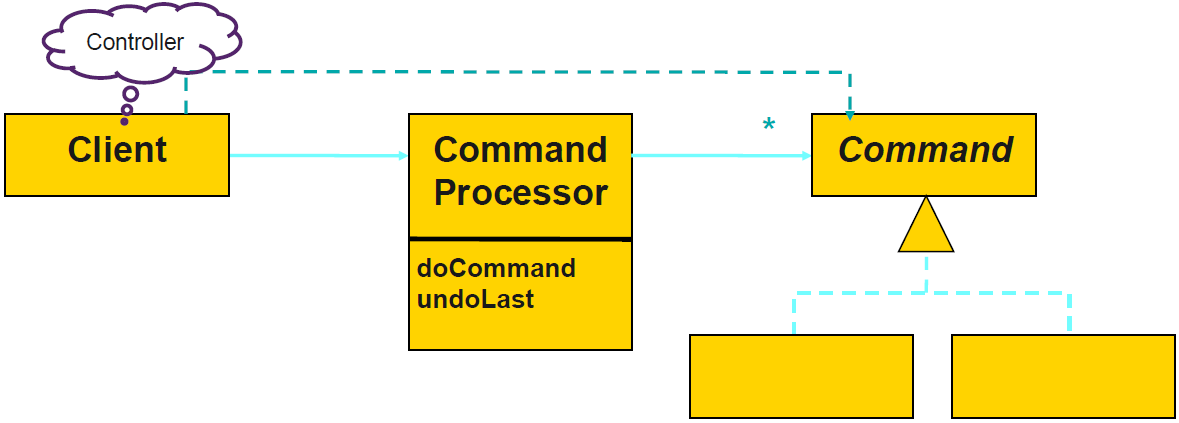
\includegraphics[width=0.8\linewidth]{./img/command_processor.png}
\textbf{Dynamics:}\\ 
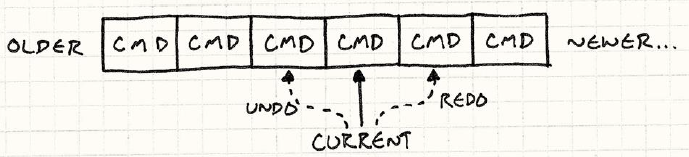
\includegraphics[width=\linewidth]{./img/command_processor_dynamic.png}
\subsubsection{Participants}
\textbf{Command Processor}
\begin{itemize}
    \item A Separate processor object can handle the responsibility for multiple Command objects
\end{itemize}
\textbf{Command}
\begin{itemize}
    \item A uniform interface to execute functions
\end{itemize}
\textbf{Controller}
\begin{itemize}
    \item Translates requests into commands and transfers commands to Command Processor.
\end{itemize}
\subsubsection{Implementation}
\begin{itemize}
    \item Command Processor contains a \textit{Stack} which holds the command history
    \item Controller creates the Commands and passes them over to Command Processor
    \item Creation of Commands may be delegated to a \textit{Simple Factory}
\end{itemize}
\subsubsection{Summary}
\textbf{Benefits:}
\begin{itemize}
    \item Flexibility
    \item Allows addition of services related to command execution
    \item Enhances testability
\end{itemize}
\textbf{Liabilities:}
\begin{itemize}
    \item Efficiency loss due additional indirection
\end{itemize}

\subsection{Visitor}
\subsubsection{Problem}
\begin{itemize}
    \item Operations on specific classes needs to be changed/added without needing to modify these classes
    \item Different algorithms needed to process an object tree
\end{itemize}
\textbf{Intent:}
\begin{itemize}
    \item How can the behaviour on individual elements of a data structure be changed/replaced whout changing the elements?
\end{itemize}
\subsubsection{Solution}
Represent an operation to be performed on the elements of an object structure. Visitor lets you define a new operation without changing the classes of the elements on which it operates.\\ 
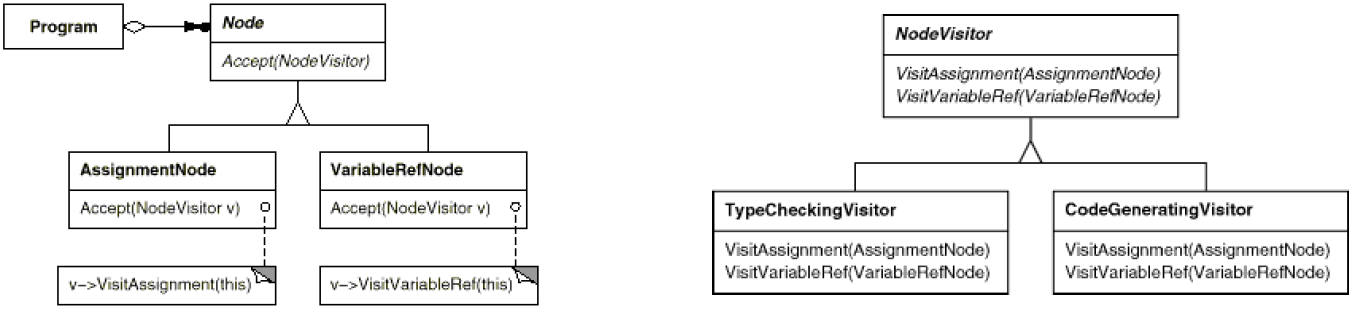
\includegraphics[width=\linewidth]{./img/visitor.png}
\subsubsection{Implementation}
\begin{itemize}
    \item 2 Class Hierarchies (Elements / Visitors)
    \item Visitors iterate though object hierarchy
    \item Solves Double-Dispatch problem of single dispatched programming languages
\end{itemize}
\textbf{Patterns that combine naturally with Vistor:}
\begin{itemize}
    \item Composite
    \item Interpreter
    \item Chain of Responsibility
\end{itemize}
\subsubsection{Summary}
\textbf{Benefits:}
\begin{itemize}
    \item Visitor makes adding new operatios easy
    \item Separates related operations from unrelated ones
\end{itemize}
\textbf{Liabilities:}
\begin{itemize}
    \item Adding new node classes is hard
    \item Visiting sequence fix defined within nodes
    \item Visitor breaks logic apart
\end{itemize}

        \section{Beyond GoF}
\subsection{External Iterator}
\subsubsection{Problem}
\begin{itemize}
    \item Iteration through a collection depends on the target implementation
    \item Separate logic of iteration into an object to allow multiple iteration strategies
\end{itemize}
\textbf{Intent:}
\begin{itemize}
    \item How can strong coupling between iteration and collection be avoided, generalized and provided in a collection-optimized manner?
\end{itemize}
\subsubsection{Solution}
Provide a way to access the elements of an aggregate object sequentially without exposing its underlying representation.\\ 
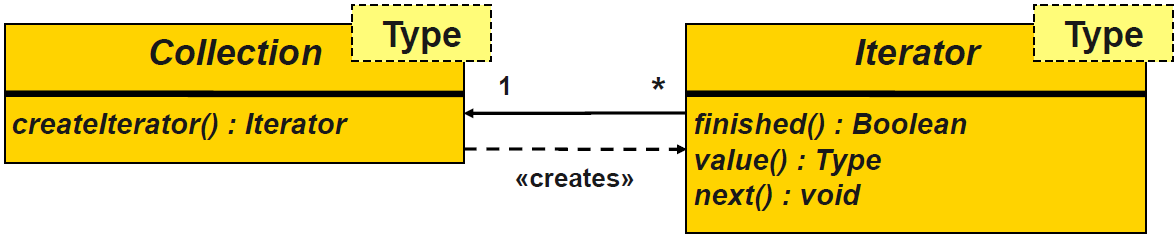
\includegraphics[width=\linewidth]{./img/external_iterator.png}
\textbf{Elementary operations of an Iterator's behaviour:}
\begin{itemize}
    \item Initializing an iteration \textit{new ArrayList().iterator();}
    \item Checking a completion condition \textit{it.hasNext();}
    \item Accessing a current target value \textit{var x = it.next();}
    \item Moving to the next target value \textit{it.next();}
\end{itemize}
\subsubsection{Summary}
\textbf{Benefits:}
\begin{itemize}
    \item Provides a single interface to loop though any kind of collection
\end{itemize}
\textbf{Liabilities:}
\begin{itemize}
    \item Multiple iterators may loop through a collection at the same time
    \item Life-Cycle Management of iterator objects
    \item Close coupling between Iterator and Collection class
    \item Indexing might be more intuitive for programmers
\end{itemize}

\subsection{Enumeration Method}
\subsubsection{Problem:}
\begin{itemize}
    \item Iteration management is performed by the collection's user
    \item Avoid state management between collection and iteration
\end{itemize}
\textbf{Intent:}
\begin{itemize}
    \item How can a collection be iterated considering the collection state and furthermore state management be reduced?
\end{itemize}
\subsubsection{Solution}
Support encapsulated iteration over a collection by placing responsibility for iteration in a method on the collection. The method takes a Command object that is applied to the elements of the collection.\\ 
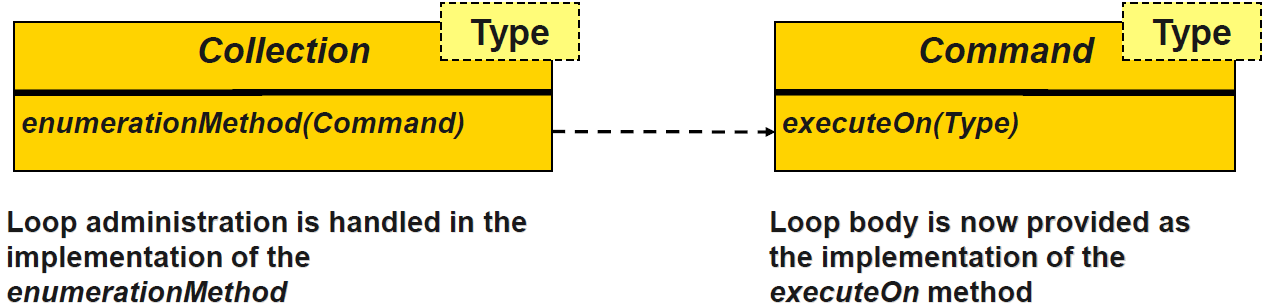
\includegraphics[width=\linewidth]{./img/enumeration_method.png}
\subsubsection{Summary}
Programming languages already implement Enumeration Method as their loop construct. (e.g. \textit{.forEach()})\\ 
\textbf{Benefits:}
\begin{itemize}
    \item Client is not responsible for loop housekeeping details
    \item Synchronization can be provided at the level of the whole traversal rather than for each element access
\end{itemize}
\textbf{Liabilities:}
\begin{itemize}
    \item Functional approach, more complex syntax needed
    \item Often considered too abstract for programmers
\end{itemize}

\subsection{Batch Method}
\subsubsection{Problem}
\begin{itemize}
    \item Collection and client (iterator user) are not on the same machine
    \item Operation invocations are no longer trivial
\end{itemize}
\textbf{Intent:}
\begin{itemize}
    \item How can a collection be iterated over multiple tiers without spending far more time in communication than in computation?
\end{itemize}
\subsubsection{Solution}
Group multiple collection accesses together to reduce the cost of multiple individual accesses in a distributed environment.
\begin{itemize}
    \item Define a data structure which groups interface calls on client side
    \item Provide an interface on servant to access groups of elements at once
\end{itemize}

\subsection{Objects for State}
\subsubsection{Problem}
\begin{itemize}
    \item Object's behaviour depends on its state, and it must change its behaviour at run-time
    \item Operations have large, multipart conditional statements (Flags) that depend on the state
\end{itemize}
\textbf{Intent:}
\begin{itemize}
    \item How can an object act according to its state without multipart conditional statements?
\end{itemize}
\subsubsection{Solution}
Allow an object to alter its behaviour when its internal state changes. The object will appear to change its class.
        \section{System Analysis}
\subsection{Individuals}
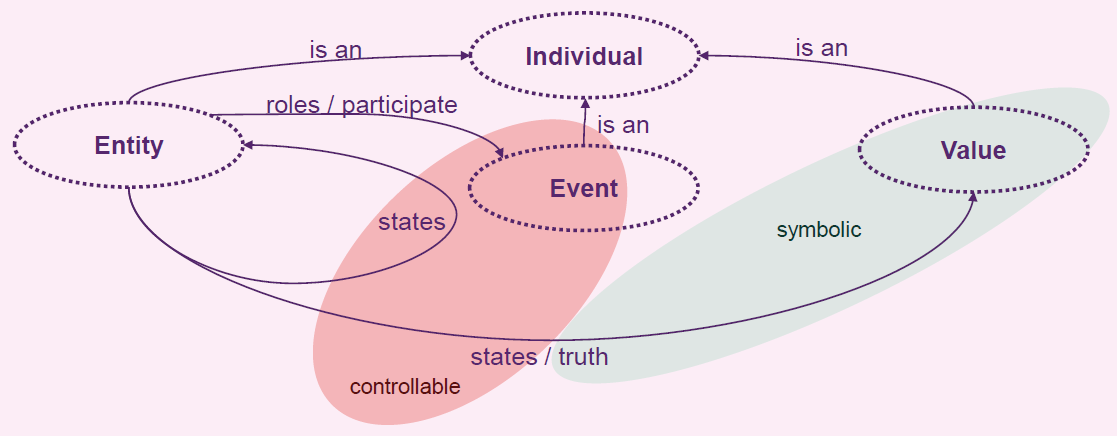
\includegraphics[width=\linewidth]{./img/value_overview.png}
\textbf{Events:}
\begin{itemize}
    \item Individual Happening, taking place at some particular point in time
    \item \textit{E.g. User-Action}
\end{itemize}
\textbf{Entities:}
\begin{itemize}
    \item Individual that persists over time and can change its properties and states.
    \item May initiate events
    \item May cause spontaneous changes to their own states
    \item May be passive
    \item \textit{E.g. Person}
\end{itemize}
\textbf{Values:}
\begin{itemize}
    \item Intangible (nicht greifbar) individual that exists outside time and space
    \item Not subject to change
    \item \textit{E.g. Körpergrösse}
\end{itemize}

\section{Software Design}
\subsection{Categories of Objects}
\textbf{Entity}
\begin{itemize}
    \item Express system information
    \item Typically persistent in nature
    \item Identity is important to distinguish entity objects
\end{itemize}
\textbf{Service}
\begin{itemize}
    \item Represent system activities
    \item Distinguished by their behaviour rather than their state
\end{itemize}
\textbf{Values}
\begin{itemize}
    \item Interpreted content is the dominant characteristic
    \item Transient and do not have significant enduring indentity
\end{itemize}
\textbf{Task}
\begin{itemize}
    \item Represent system activities
    \item Have an element of identity and state
\end{itemize}

\section{Object Aspects}
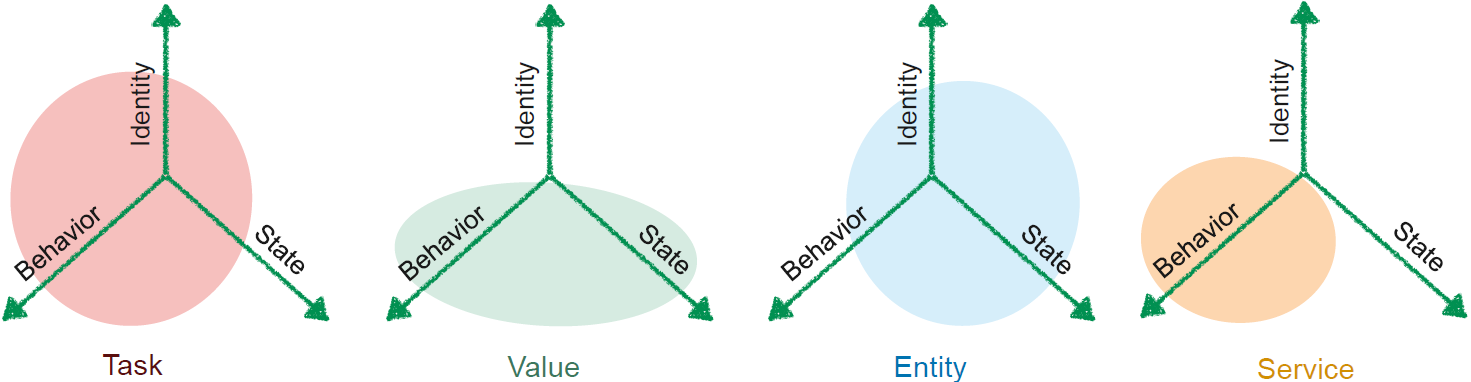
\includegraphics[width=\linewidth]{./img/object_aspects.png}

\section{Value Objects}
\begin{itemize}
    \item Usually do not appear in UML class diagrams (except attribute type)
    \item Model fine-grained information
    \item Contain repetitive common code
    \item Used to add meaning to primitive value types
    \item Ensure type safety
    \item \textit{E.g. IBAN Type Object (10 digits, checksum)}
\end{itemize}

\section{Value patterns}
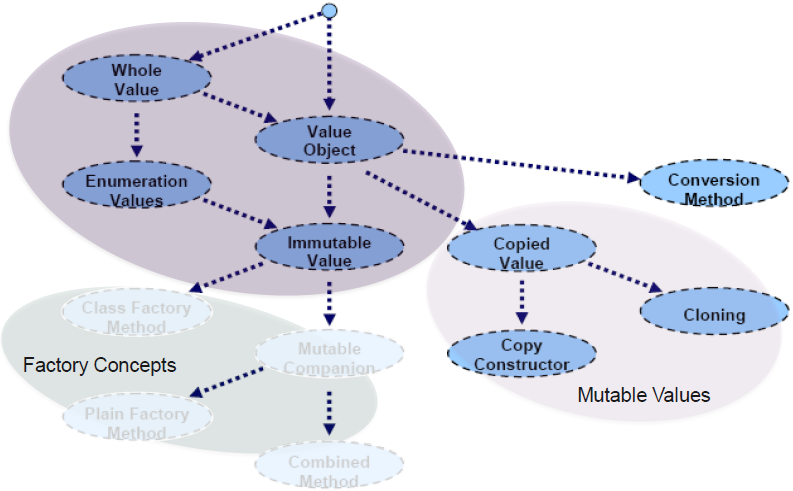
\includegraphics[width=\linewidth]{./img/value_pattern_overview.png}

\subsection{Whole Value}
\subsubsection{Problem}
\begin{itemize}
    \item Plain integers and floating-point numbers are not very useful as domain values
    \item Errors in dimension and intent communication should be addressed at complile time
    \item How can you represent primitive quantities from your proble domain without loss of meaning?
\end{itemize}
\subsubsection{Solution}
Express the type of the quantity as a Value Class.\\ 
\begin{itemize}
    \item Recovers the loss of meaning and checking by providing a \textbf{dimension} and \textbf{range}
    \item Wraps simple types or attribute stes
    \item Disallows inheritance to avoid slicing
    \item \textit{E.g. Year, Month, Day Classes for Dates}
\end{itemize}
\begin{lstlisting}
public final class Date {
    public Date(Year year, Month month, Day day) { ... }
}
\end{lstlisting}

\subsection{Value Object / Value Class}
\subsubsection{Problem}
\begin{itemize}
    \item Comparison, indexing and ordering should not rely on objects identity but its content
    \item How do you define a class to represent values in your system?
\end{itemize}
\subsubsection{Solution}
Override methods in Object whose action should be related to content and not identity and implement serializable.\\
\begin{itemize}
    \item Override Object's methods who define equality
    \item Java
    \begin{itemize}
        \item \textit{equals(Object other)}
        \item \textit{hashCode()}
        \item implement \textit{Serializable / toString()} if appropriate
    \end{itemize}
    \item TypeScript
    \begin{itemize}
        \item \textit{equals(other: Object)}
        \item implement \textit{toString()} if appropriate
    \end{itemize}
    \item Overriding \textit{toString()} can help using your Value Object
\end{itemize}

\subsection{Conversion Method}
\subsubsection{Problem}
\begin{itemize}
    \item Values are strongely informational objects without a role for separate identity
    \item Often Value Objects are somehow related but cannot be used directly without conversion
    \item How could you use different, related Value Objects together without depending on underlying primitive type?
\end{itemize}
\subsubsection{Solution}
Provide type conversion methods responsible for converting Value Objects into related formats.
\begin{itemize}
    \item Provide a constructor which converts between types\\\textit{String(char[] value)}
    \item Or create a conversion instance method that converts to other type \\\textit{Date.toOtherType()}
    \item Or create a \textbf{Class Factory Method} with conversion characteristics \\\textit{Date.from(Instant i)}
\end{itemize}

\subsection{Immutable Value}
\subsubsection{Problem}
\begin{itemize}
    \item A value exists outside time and space and is not subject to change
    \item Avoid side effect problems when sharing Value Objects
    \item Sharing values across Threads requires thread safety
    \item Values are often threaded as key for associative tables
    \item How can you share Value Objects and guarantee no side effect problems?
\end{itemize}
\subsubsection{Solution}
Set the internal state of the Value Class object at construction and allow no modifications.\\ 
\begin{itemize}
    \item Declare all fields private final
    \item Mark class as final
    \item No Syncrhonization needed
\end{itemize}

\subsection{Enumeration Values}
\subsubsection{Problem}
\begin{itemize}
    \item A fixed range of values should be typed \textit{e.g. months}
    \item Using just int constants doesn't help
    \item Whole Value is only half the solution; range should be constant
    \item How can you represent a fixed set of constant values and preserve type safety?
\end{itemize}
\subsubsection{Solution}
Treat each constant as Whole Value instance declaring it public.
\begin{itemize}
    \item Implement a Whole Value and declare the Enumeration Values as \textit{public readonly} fields
    \item Prevent inadvertently changing the constants
    \item Pattern is built in (enum)
\end{itemize}

\subsection{Copied Value and Cloning}
\subsubsection{Problem}
\begin{itemize}
    \item Values should be modifiable without changing the origins internal state
    \item How can you pass a modifiable Value Object into and out of methods without permitting callers or called methods to affect the original object?
\end{itemize}
\subsubsection{Solution}
Implement Cloneable interface to be used whenever a value object needs to be returned or passed as a parameter.
\begin{itemize}
    \item Clone every Value Object leaked across boundaries (parameters / return values)
    \item May result in immense object creation overhead (cloning is expensive)
    \item Imitates \textit{call-by-value} and \textit{return-by-value}
\end{itemize}

\subsection{Copy Constructor}
\subsubsection{Problem}
\begin{itemize}
    \item Within Value Objects we often know exactly what to copy
    \item How can objects be copied without the need of implementing a clone method?
\end{itemize}
\subsubsection{Solution}
Provide a way to construct an object based on another instance with exactly the same type.
\begin{itemize}
    \item Declare the class \textit{final} and derive from Object only
    \item Create a copy constructor, which consumes an instance with same type
\end{itemize} 
\begin{lstlisting}
public final class Date {
    public Date(Date other) {
        // ... 
        this.year = new Year(other.year);
    }
}
\end{lstlisting}

\subsection{Class Factory Method / Simple Factory}
\subsubsection{Problem}
\begin{itemize}
    \item Construction of Value Objects may be expensive
    \item Different construction logic is required which may result in huge amount of constructors
    \item How can you simplify and potentially optimize construction of Value Objects in expressions without introducing new intrusive expressions?
\end{itemize}
\subsubsection{Solution}
Provide static methods to be used instead of ordinary constructors. The methods return either newly created Value Objects or cached Objects.
\begin{itemize}
    \item Declare one or more creation method on the class
    \item Define constructors \textit{private}, they are invoked by Class Factory Method
    \item The static methods could also contain caching mechanisms
\end{itemize}
\begin{lstlisting}
public final class Year {
    public static Year of(int value) {
        return new Year(value);
    }
    private Year(int value) { this.value = value; }
}
\end{lstlisting}

\subsection{Mutable Companion}
\subsubsection{Problem}
\begin{itemize}
    \item We need to calculate with alues \textit{e.g. 15 working days after exam}
    \item How can you simplify complex construction of an immutable value?
\end{itemize}
\subsubsection{Solution}
Implement a companion class that supports modifier methods and acts as a factory for immutable Value Objects.
\begin{itemize}
    \item Factory Object for immutable values
    \item Neither a subtype nor a supertype of the Immutable Value
\end{itemize}
\begin{lstlisting}
public final class YearCompanion {
    private int value;
    public YearCompanion(Year toModify) { this.value = toModify.getValue(); }
    /* modifying methods */
    public Year asValue() { /* Factory Method */
        return Year.of(value);
    }
}
\end{lstlisting}

\subsection{Relative Values}
\subsubsection{Problem}
\begin{itemize}
    \item Value Objects are compared by their state, not their identity
    \item Relative comparison between Value Objects for appropriate values should be provided
    \item How can a Value Obejct be compared against others in a typed way?
\end{itemize}
\subsubsection{Solution}
Implement the responsibility for comparison between Value Objects by deriving from \textit{Comparable} interface.
\begin{itemize}
    \item Override-Overload Method Pair: (\textit{compareTo(T other)} and \textit{equals(T other)})
    \item Bridge Method: Provide a Method for \textit{equals(Object other)} and forward it to \textit{equals(T other)}
    \item 
\end{itemize}

\subsection{Discussion}
\textbf{Difference between Whole Value and Immutable Value}
\begin{itemize}
    \item Whole: Value with a unit should be encapsulated in a class
    \item Immutable: Value within an object must be immutable
\end{itemize}
\textbf{When would you prefer Class Factory Method over a conversion constructor?}
\begin{itemize}
    \item Factory: A foreign value type should be converted into the current value format
    \item Contructor: A more generic type should be converted into the current type
\end{itemize}
\textbf{What are the most important liabilities of the Mutable Value concept?}
\begin{itemize}
    \item Concept of Cloning / Copied Value may be missed by the programmer which results in to hard to find errors
\end{itemize}
        \section{Checks}
\begin{itemize}
    \item Separate good input from bad
    \item Information integrity checks
    \item Applied without complicating the program
\end{itemize}
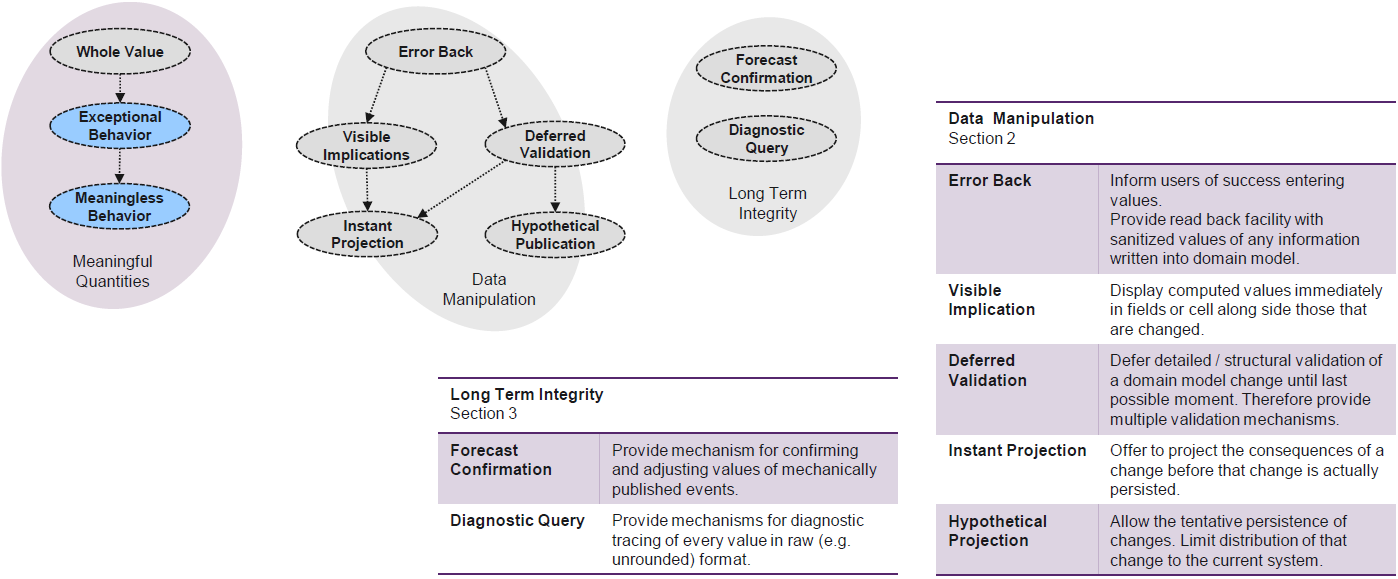
\includegraphics[width=\linewidth]{./img/checks_overview.png}

\subsection{Exceptional Behaviour}
\subsubsection{Problem}
\begin{itemize}
    \item Missing or incorrect values in a domain model are impossible to avoid
    \item The domain logic should be able to handle this sort of missing data
    \item How can exceptional behaviour caused by invalid input be handled without throwing errors?
\end{itemize}
\subsubsection{Solution}
Use one or more distinguished values to represent exceptional circumstances.
\begin{itemize}
    \item Invalid parametrized domain calls may produce Exceptional Values
    \item Domai logic may accept Exceptional Value as legal input
\end{itemize}
\begin{lstlisting}
// TypeScript
public div(num: number, div: number): number | CalcError {
    div === 0 ? CalcError.DivByZero : num / div;
}
\end{lstlisting}

\subsection{Meaningless Behaviour}
\subsubsection{Problem}
\begin{itemize}
    \item Due to error handling, domain logic may be expressed with more complexity than originally conceived
    \item How can exceptional behaviour due to invalid input be handled without throwing errors?
\end{itemize}
\subsubsection{Solution}
Write methods with minimalistic concern for possible failure.
\begin{itemize}
    \item Initiate computation
    \item If it fails:
    \begin{itemize}
        \item recover from failure and continue processing
        \item ensure the error is logged/visualized on surface
    \end{itemize}
    \item Choose meaningless behaviour unless a condition has domain meaning 
    \item Represents an alternative implementation of Exceptional Value
\end{itemize}
\begin{lstlisting}
// TypeScript
public div(num: number, div: number): number {
    return num / div; // Infinity (Java NaN) if div == 0
}
\end{lstlisting}

\section{Framework Introduction}
\textbf{Why Frameworks}
\begin{itemize}
    \item Avoid re-inventing the wheel
    \item It is easy but inefficient to program the same thing again and again
\end{itemize}
\textbf{What is a Framework}
\begin{itemize}
    \item Object-Oriented classes that work together
    \item Framework provides \textit{hooks} for extension
    \item In contrast to a library, a framework keeps the control flow, not your extension
    \item Inversion of control via callbacks
\end{itemize}
\textbf{Framework Callbacks}
\begin{itemize}
    \item Hollywood Principle: Don't call us, we call you!
    \item Extendability and configurability
\end{itemize}
\subsection{Application Framework}
\begin{itemize}
    \item Object-oriented class library
    \item \textit{Main()} program lives in the Application Framework
    \item Provides \textit{hooks} and \textit{callbacks}
    \item Provides ready-made classes for use
    \item Creates product families
    \item Reuse of application architecture and infrastructure
\end{itemize}
\subsection{Examples}
\textbf{Frameworks}
\begin{itemize}
    \item .NET Core
    \item Entity Framework
    \item React (lib)
    \item Vue
\end{itemize}
\textbf{Application Framework}
\begin{itemize}
    \item Spring
    \item ASP.NET
    \item Angular
\end{itemize}

\subsection{Difference: Library / Framework / App Framework}
\textbf{Library}
\begin{itemize}
    \item Contain 3rd party Features which do not control the app flow (e.g. Math Library)
\end{itemize}
\textbf{Framework}
\begin{itemize}
    \item Provide Hooks / Extension points
    \item Strogly rely on Inversion of Control (IoC)
    \item Defines when hooks are called, thus controlls part of the app flow
\end{itemize}
\textbf{App Framework}
\begin{itemize}
    \item Contains the \textit{main()} procedure
    \item Completely controlls the app flow
\end{itemize}

\subsection{Summary}
\textbf{Benefits}
\begin{itemize}
    \item Less code to write
    \item Reliable and robust code
    \item Consistent and modular code
    \item Reusability
    \item Maintenance
\end{itemize}
\textbf{Liabilities}
\begin{itemize}
    \item Portability: Code is strongly coupled to the overlying Framework 
    \item Testing: Close coupling between framework parts
    \item Evolution: User's implemetation may break due next Framework version
\end{itemize}

\subsection{Hook / Extension Point / Control Flow}
\subsubsection{Template Method}
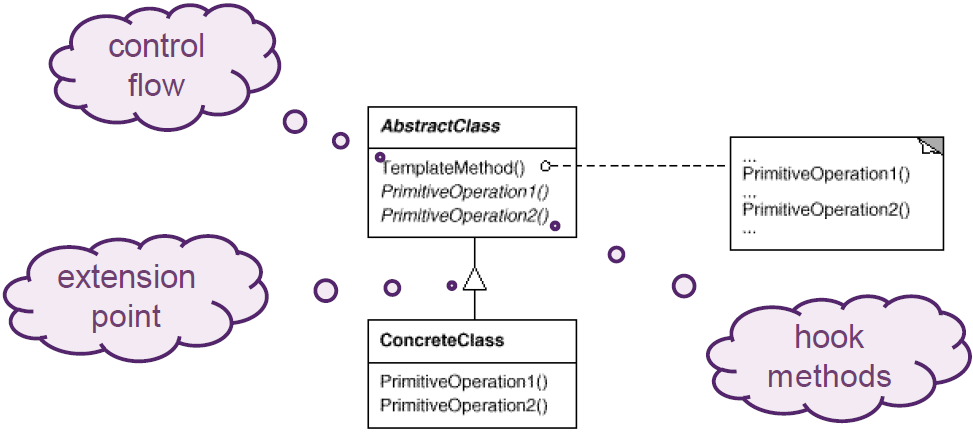
\includegraphics[width=\linewidth]{./img/template_method_example.png}
\subsubsection{Strategy}
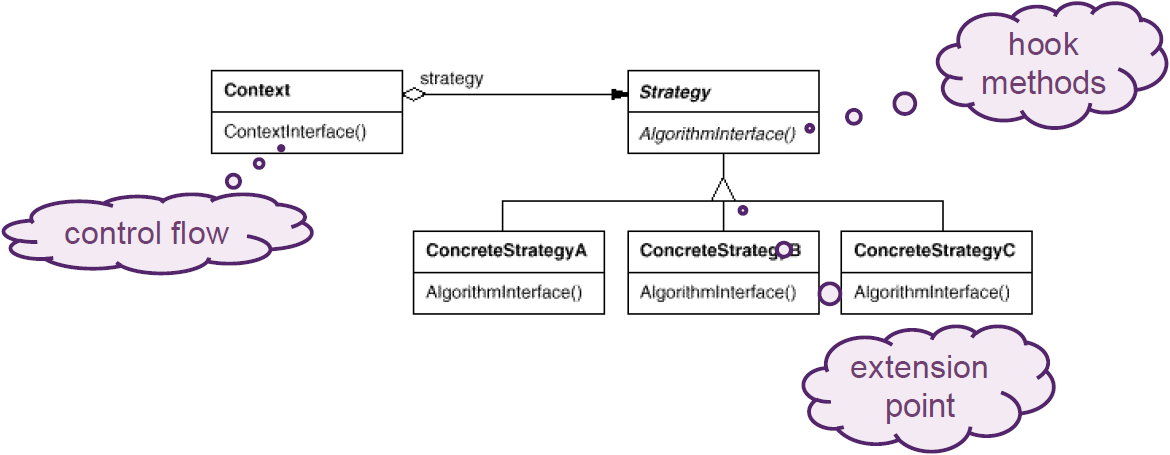
\includegraphics[width=\linewidth]{./img/strategy_example.png}
\subsubsection{Command Processor}
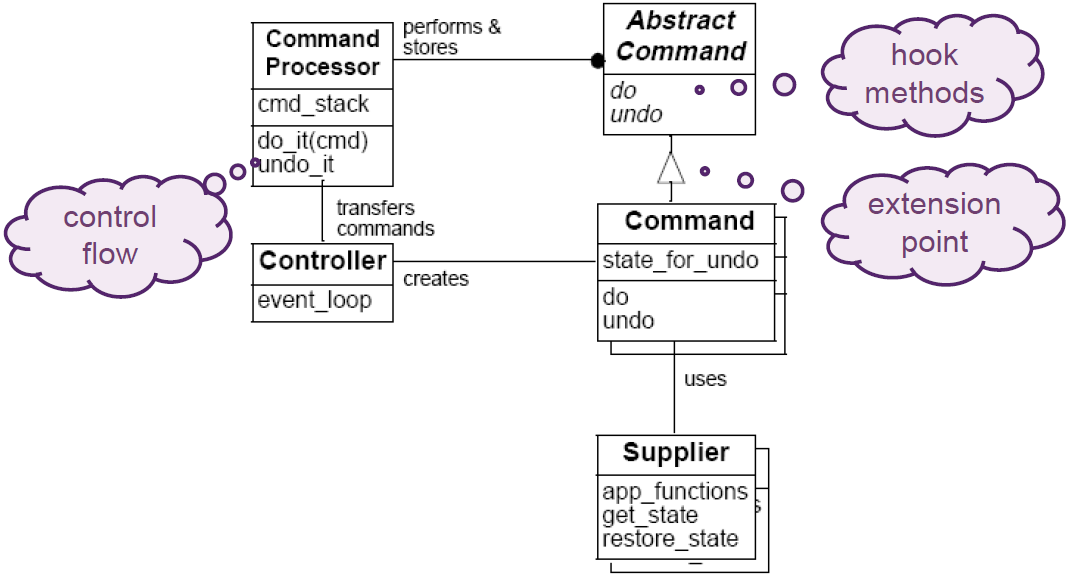
\includegraphics[width=\linewidth]{./img/command_processor_example.png}
\subsubsection{Flyweight}
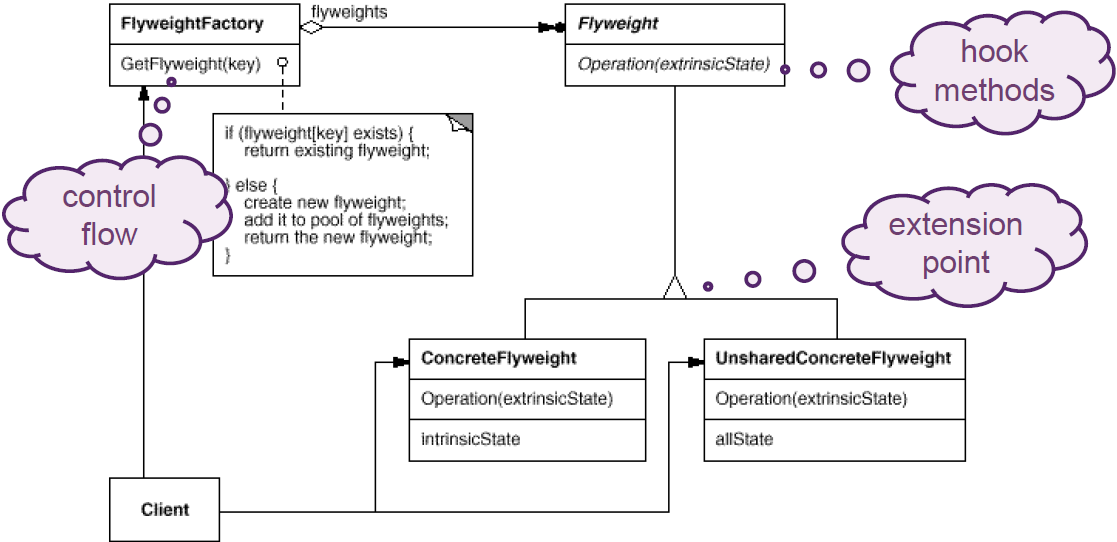
\includegraphics[width=\linewidth]{./img/flyweight_hooks.png}



\section{Meta Frameworks}
A Framework for Evaluating Software Technology
\begin{itemize}
    \item Initial acquisition cost
    \item Long-term effect
    \item Training and support
    \item Future technoloy plans
    \item Response of direct competitor organizations
\end{itemize}

\subsection{Framework Evaluation Phases}
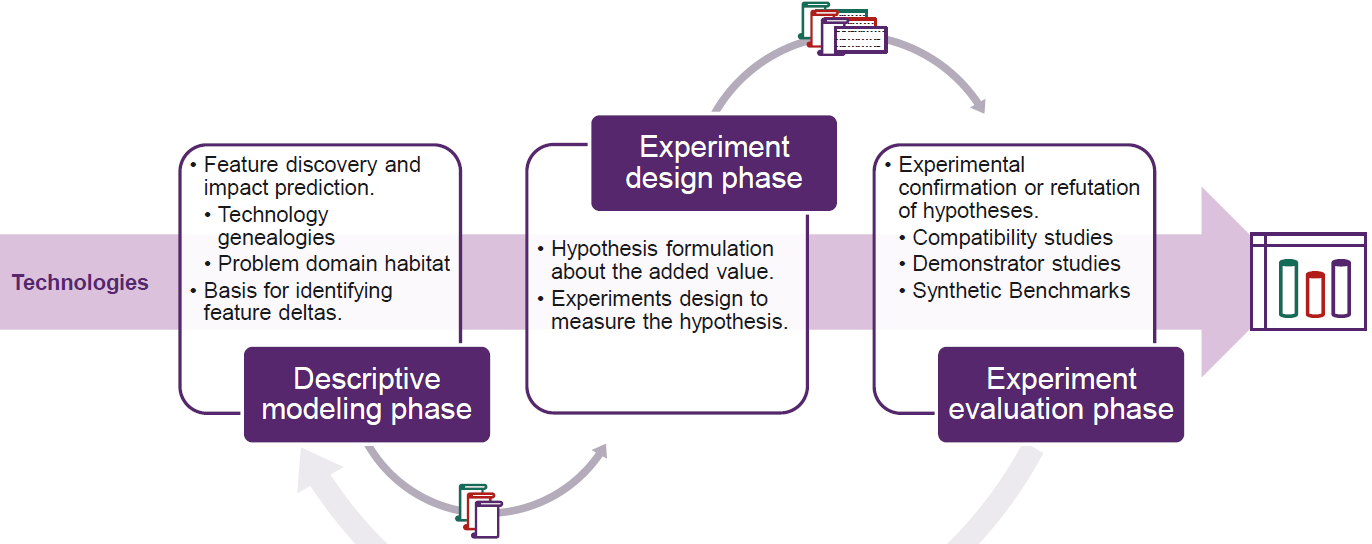
\includegraphics[width=\linewidth]{./img/framework_eval.png}

\section{Developing Frameworks}
\begin{itemize}
    \item Frameworks need evolutionary improvements
\end{itemize}
\subsubsection{Frameworkers Dilemma}
\textbf{Potential ways out of the dilemma}
\begin{enumerate}
    \item Think very hard up-front
    \item Don't care too much about framework users
    \item Let framework users participate
    \item Use helping technology
\end{enumerate}
        \section{Meta Pattern}
\begin{itemize}
    \item Reflection is often used as technology for Meta Programming
    \item Provide Flexibility, Adaptability \& Generality
\end{itemize}
\textbf{Recurring Problems}
\begin{itemize}
    \item Reflection solves common frameworkers problems
    \item Exchanging parts of a software system is hard
    \item Not yet unknown sofware components should be integrated
\end{itemize}

\subsection{Reflection}
\textbf{Usage (Java / C\#)}
\begin{itemize}
    \item Load of JAR / DLL
    \item Invoke Methods 
    \item Read out properties/fields 
    \item Create object instances 
    \item Search for annotations on Classes / Methods / Fields / ...
\end{itemize}
\textbf{Provides Facility to implement:}
\begin{itemize}
    \item DI
    \item Convention over Configuration
    \item Object-Relation Mapper
    \item Serialization / Deserialization
    \item Plugin Architectures
\end{itemize}
Consists of two aspects:\\ 
\textbf{Introspection}
\begin{itemize}
    \item The ability for a program to observe and therefore reason about its own state
    \item e.g. Query object properties, get list of methods
\end{itemize}
\textbf{Intercession}
\begin{itemize}
    \item The ability of a program to modify its own execution state or alter its own interpretation of meaning
    \item e.g. Modify object properties, add another attribute or exchange code
\end{itemize}
Defines meta level and base level:\\ 
\textbf{Meta level}
\begin{itemize}
    \item Provides self-representation
    \item Gives the SW a knowledge of its own structure
    \item Consists of meta objects
\end{itemize}
\textbf{Base level}
\begin{itemize}
    \item Defines the app logic
    \item Implementation may use the meta objects
\end{itemize}
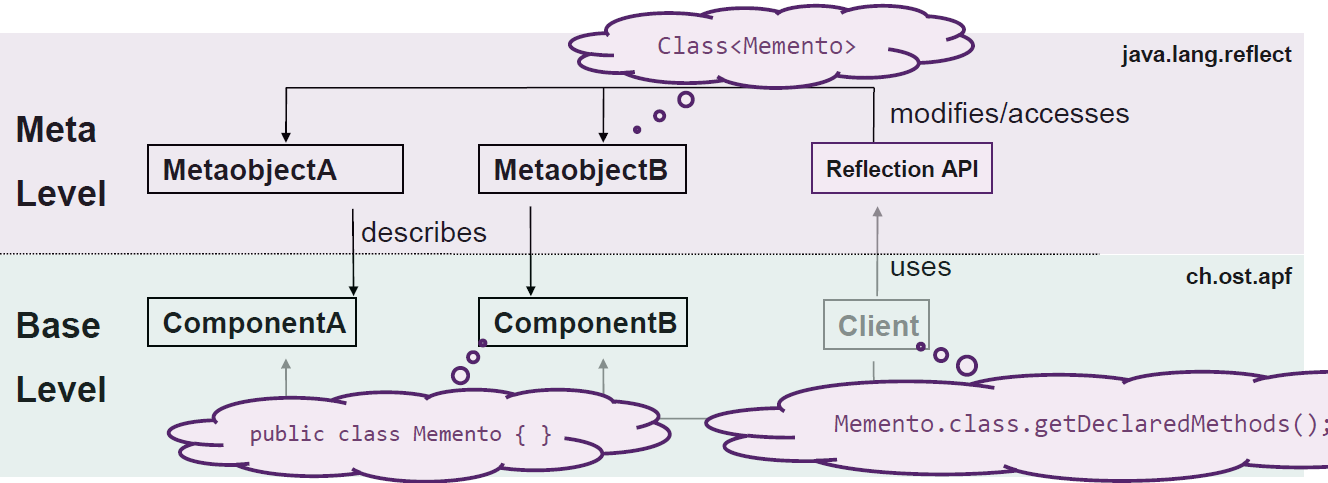
\includegraphics[width=\linewidth]{./img/meta_base_level.png}
\subsubsection{Summary}
\textbf{Benefits}
\begin{itemize}
    \item Adapting a software system is easy
    \item Support for many kinds of changes
\end{itemize}
\textbf{Liabilities}
\begin{itemize}
    \item Produces non-transparent APIs
    \item Binding at runtime (limited Type safety)
\end{itemize}

\subsection{Meta Objects}
\textbf{Usage}
\begin{itemize}
    \item Classes
    \item Object Attributes
    \item Methods
    \item Class Relationships
\end{itemize}

\subsection{Type Object}
\subsubsection{Problem}
\begin{itemize}
    \item We want to keep common behaviour and data in only one place
    \item DRY implementation of domain
    \item How can you categorize objects, eventually dynamically?
\end{itemize}
\subsubsection{Solution}
Categorize objects by another object instead of a class. Thus an object can change it's 'class' at runtime
\begin{itemize}
    \item Create a category (type) object which describes multiple objects
    \item Objects forward the calls to the underlying type
\end{itemize}
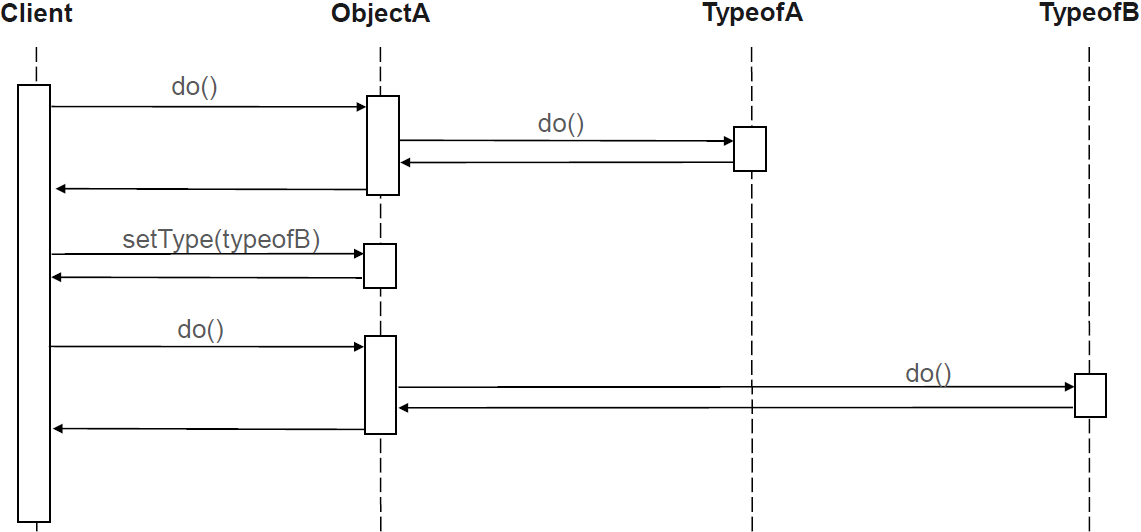
\includegraphics[width=\linewidth]{./img/type_object.png}
\subsubsection{Summary}
\textbf{Benefits}
\begin{itemize}
    \item Categories can be added easily, event at runtime
    \item Allows multiple meta-levels
\end{itemize}
\textbf{Liabilities}
\begin{itemize}
    \item Confusing mess of 'classes' because of separation
    \item Lower efficiency because of indirection
    \item Changing database schemas can be tricky
\end{itemize}
\subsubsection{Discussion}
\textbf{Based on which GoF Pattern}
\begin{itemize}
    \item Strategy
\end{itemize}
\textbf{Similar intent in a GoF Pattern}
\begin{itemize}
    \item State, also changes at runtime
\end{itemize}

\subsection{Property List}
\subsubsection{Problem}
\begin{itemize}
    \item Attributes should be attachable / detachable after compilation
    \item Objects share attributes / parameters across the class hierarchy
    \item How do you define properties in a flexible way so they can be attached and detached at runtime?
\end{itemize}
\subsubsection{Solution}
Provide objects with a property list. That list allows to associate names with other values or objects.
\begin{itemize}
    \item Property list maps attribute names to values
    \item each name defines a slot
    \item Same slot can be used for attributes with identical semantics
    \item Objects can be triggred to list all slot names and values
\end{itemize}
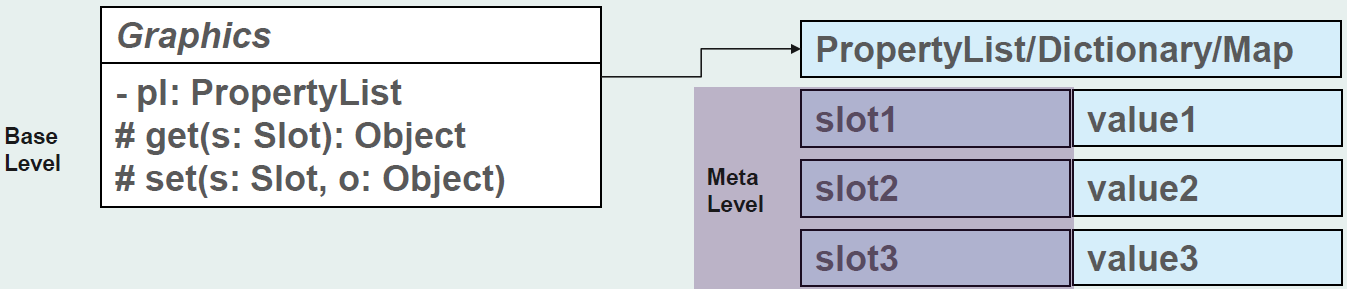
\includegraphics[width=\linewidth]{./img/property_list.png}
\subsubsection{Summary}
\textbf{Benefits}
\begin{itemize}
    \item Attributes can be added dynamically
    \item Object extension while keeping object identity
    \item Easy attribute iteration
\end{itemize}
\textbf{Liabilities}
\begin{itemize}
    \item Different ways to access regular / dynamic attributes
    \item Type safety left to the programmer
    \item Run-time overhead
    \item Memory Management
\end{itemize}
\textbf{Mitigate Liabilities:} Bridge Methods

\subsection{Anything}
\begin{itemize}
    \item Arbitrary data structure
    \item Recursively structured Property List
    \item Internal representation of today's JSON
\end{itemize}
\textbf{Object Definition:}
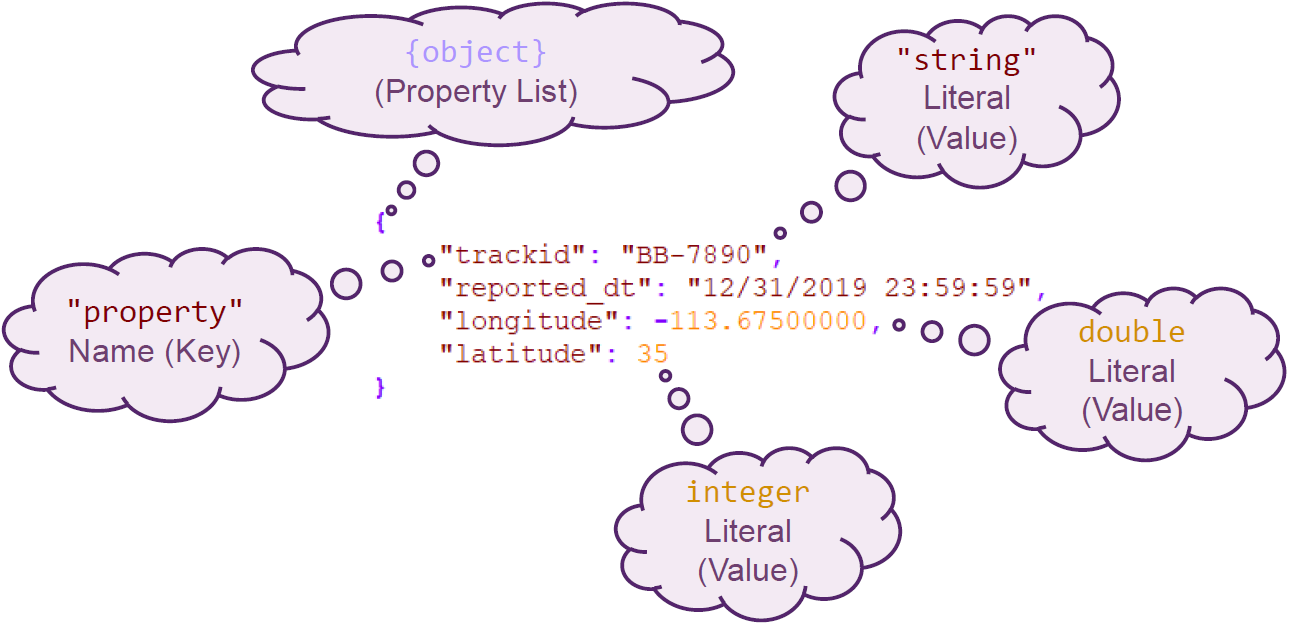
\includegraphics[width=\linewidth]{./img/anything.png}
\subsubsection{Problem}
\begin{itemize}
    \item We need to keep a map of data similar to the Property List
    \item Structured data also includes sequences of data
    \item Data should be structured recursively
    \item How do you provide a generic configuration or communication data structure that is easily extensible?
\end{itemize}
\subsubsection{Solution}
Create an abstraction for structured values that is self describing.
\begin{itemize}
    \item Implement a representation of simple values
    \item Add an implementation for a sequence of values (\& key value access)
    \item Provide a default value
\end{itemize}
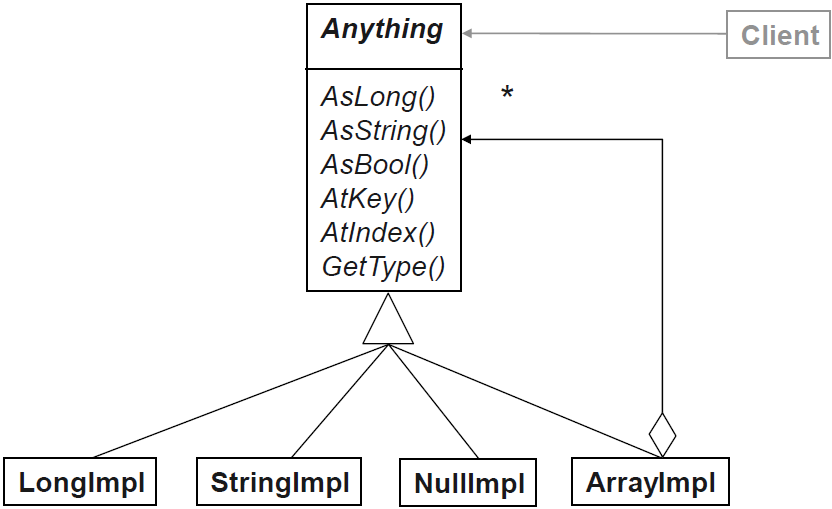
\includegraphics[width=\linewidth]{./img/anything_uml.png}
\subsubsection{Summary}
\textbf{Benefits}
\begin{itemize}
    \item Readable streaming format
    \item Appropriate for configuration data
    \item Universally applicable
    \item Flexible interchange across class/object boundaries
\end{itemize}
\textbf{Liabilities}
\begin{itemize}
    \item Less type safety
    \item Intent of parameter elements not always obvious
    \item Overhead for value lookup and member access
    \item No real object, just data
\end{itemize}
\subsubsection{Discussion}
\textbf{Which GoF Pattern does Anything implement?}
\begin{itemize}
    \item Transparent Composite Pattern
    \item Null Object
\end{itemize}

        \section{Reimplementing React}
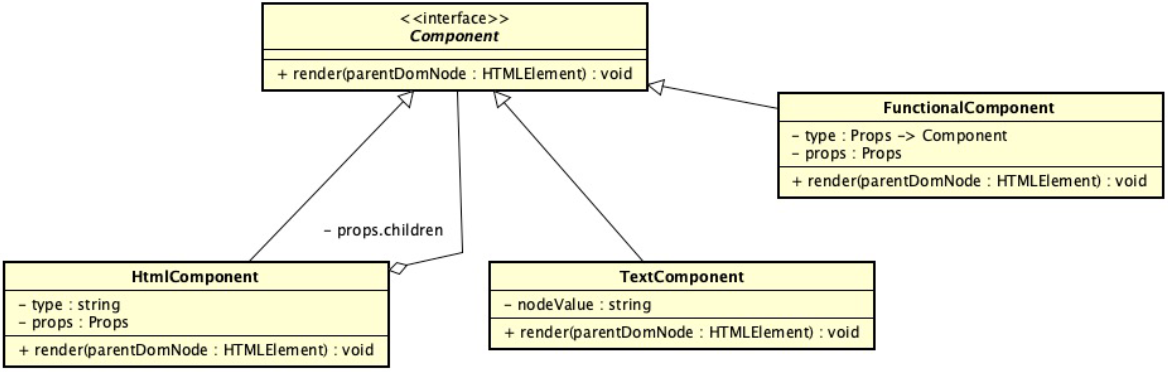
\includegraphics[width=\linewidth]{./img/react_types.png}\\
Code????
\vspace{0.5cm}
\section{Reimplementing Redux}
\vspace{0.5cm}
Code???
\vspace{0.5cm}


        \section{Eclipse}
\subsection{Components}
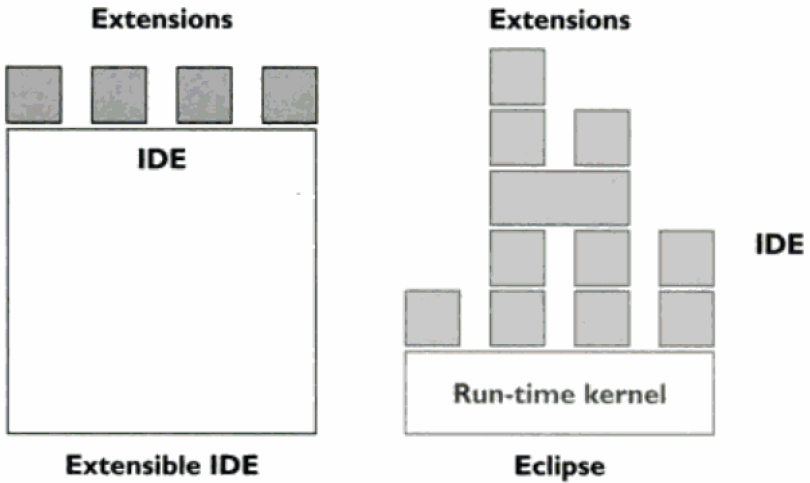
\includegraphics[width=0.7\linewidth]{./img/eclipse_components.png}
\subsubsection{SWT}
\begin{itemize}
    \item Native Widgets and mostly written in Java
    \item No performance implact form UI
    \item Provides basic Components
\end{itemize}
\subsubsection{JFace}
\begin{itemize}
    \item Builds on top of SWT 
    \item Actions 
    \item Menus 
    \item Dialogs 
    \item Wizards 
    \item Fonts 
\end{itemize}
\subsubsection{OSGi}
\begin{itemize}
    \item Specifies a component and service model for Java
    \item Components can be installed, started, stopped and uninstalled at runtime 
    \item Each bundle gets its own classloader
    \item Bundles define dependencies and export some of their packages
\end{itemize}
\textbf{Bundles:}
\begin{itemize}
    \item Eclipse Plugins are OSGi Bundles
    \item Packaged as JARs
    \item MANIFEST.MF contains the bundle metadata
\end{itemize}
\textbf{Services:}
\begin{itemize}
    \item Connect Bundles
    \item Service is a POJO and can be registered at a Service Registry at bundle start
    \item Eclipse does not use OSGi services but Extensions and Extension Points
\end{itemize}

\subsubsection{Extension Points}
\begin{itemize}
    \item Collect contributions to the plug-in offering the Extension Point 
    \item Each plug-in contributes to at least one extension point
    \item EP and Extensions are not part of the Manifest but separate XML files
\end{itemize}
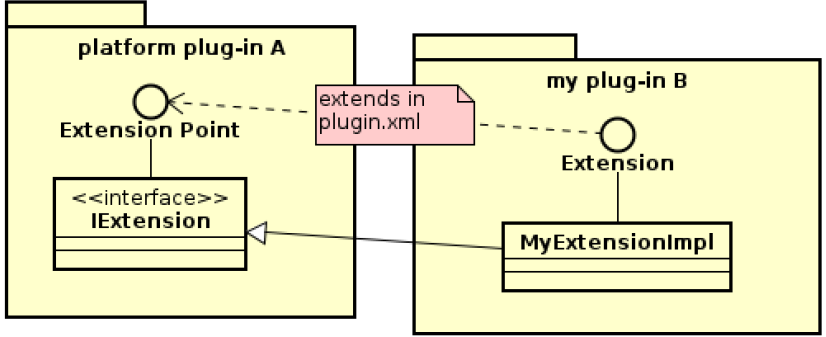
\includegraphics[width=0.7\linewidth]{./img/ep.png}

\subsection{Eclipse Plug-ins}
\begin{itemize}
    \item Add new Actions, Editors, Views, Perspectives, Preferences
    \item Each one gets its own class loader
    \item Can only access specified dependencies
    \item Has three interesting files
    \begin{itemize}
        \item Manifest
        \item plugin.xml: wires up the Extension
        \item Class that imlements the Extension
    \end{itemize}
\end{itemize}
\textbf{Eclipse Platform}
\begin{itemize}
    \item Manages Plugins
    \item Discover installed plug-ins
    \item builds the extension registry
    \item connects extesions and EP
    \item Only activates plug-ins when needed
\end{itemize}

\subsection{GoF Design Patterns in Eclipse}
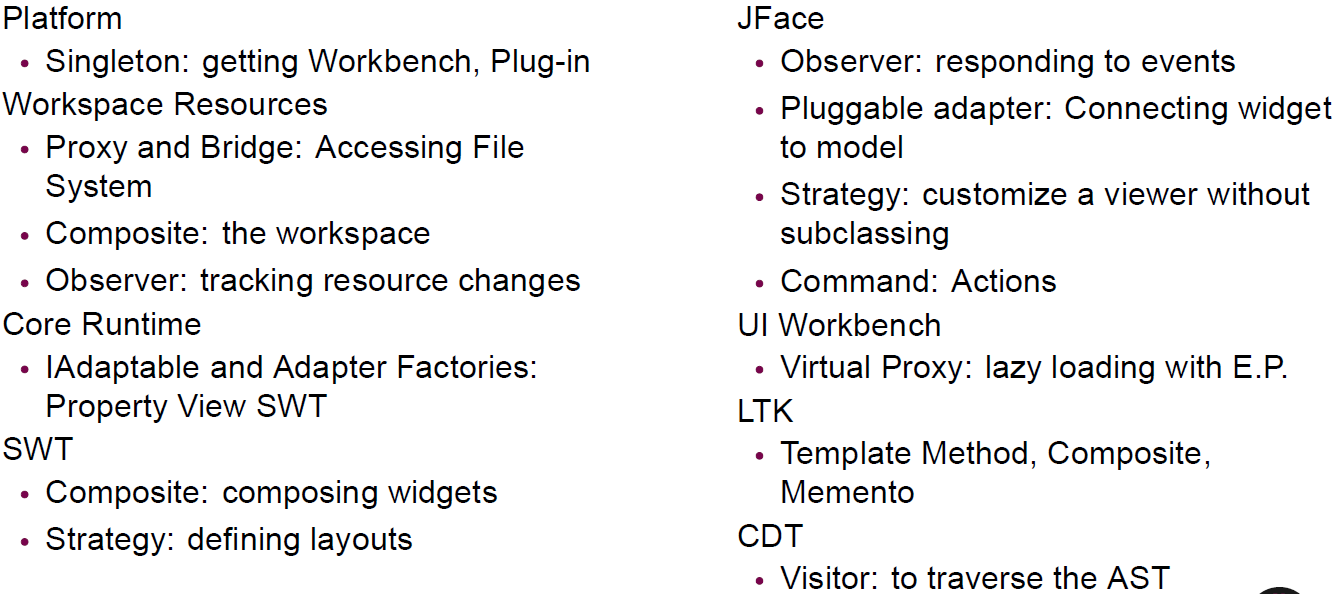
\includegraphics[width=\linewidth]{./img/eclipse_gof.png}

\subsection{Refactoring Language Toolkit (LTK)}
\begin{itemize}
    \item Language neutral API for refactorings
    \item Classes for constructing refactoring UI (common L\&F for wizards)
    \item Refactoring wizard with diff preview
    \item Classes for modelling resource changes
    \item Refactoring participant functionality
\end{itemize}
\subsubsection{Refactoring Lifecycle Overview}
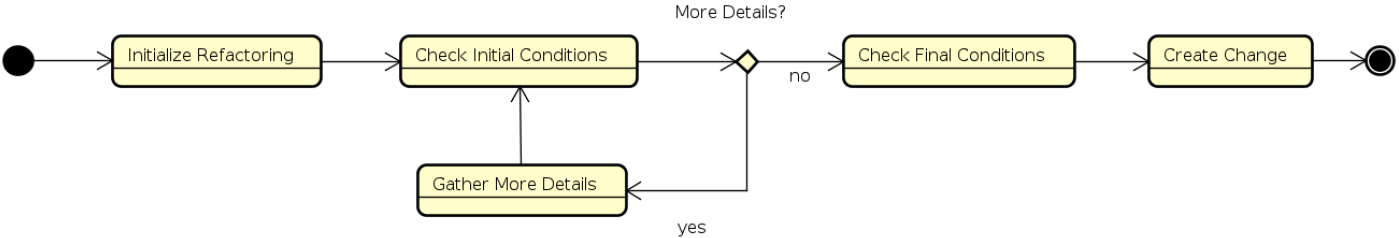
\includegraphics[width=\linewidth]{./img/refactoring_lc.png}

\subsubsection{Refactoring Participants}
\begin{itemize}
    \item Can participate in the condition checking and change creation of a refactoring processor
    \item Refactorings that change multiple files may have an impact on other tools
\end{itemize}


        \section{Spring Framework}
Provides a programming and configuration model for modern Java-based enterprise applications - on any kind of deployment platform.

\subsection{Java Annotations}
\begin{itemize}
    \item Metadata that do not directly affect the code they annotate
    \item Uses
    \begin{itemize}
        \item Information for the compiler
        \item Compile-time and deployment-time proccessing
        \item Runtime processing
    \end{itemize}
\end{itemize}
\subsubsection{Examples}
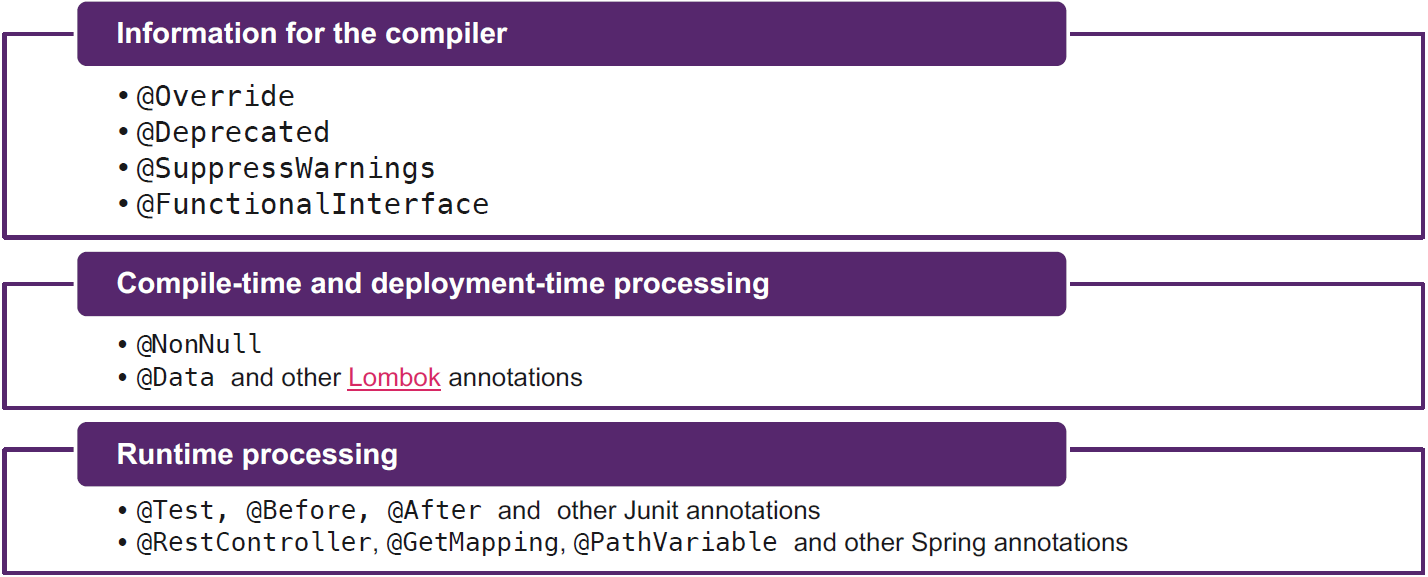
\includegraphics[width=\linewidth]{./img/annotation.png}
\subsubsection{Declaring Annotations}
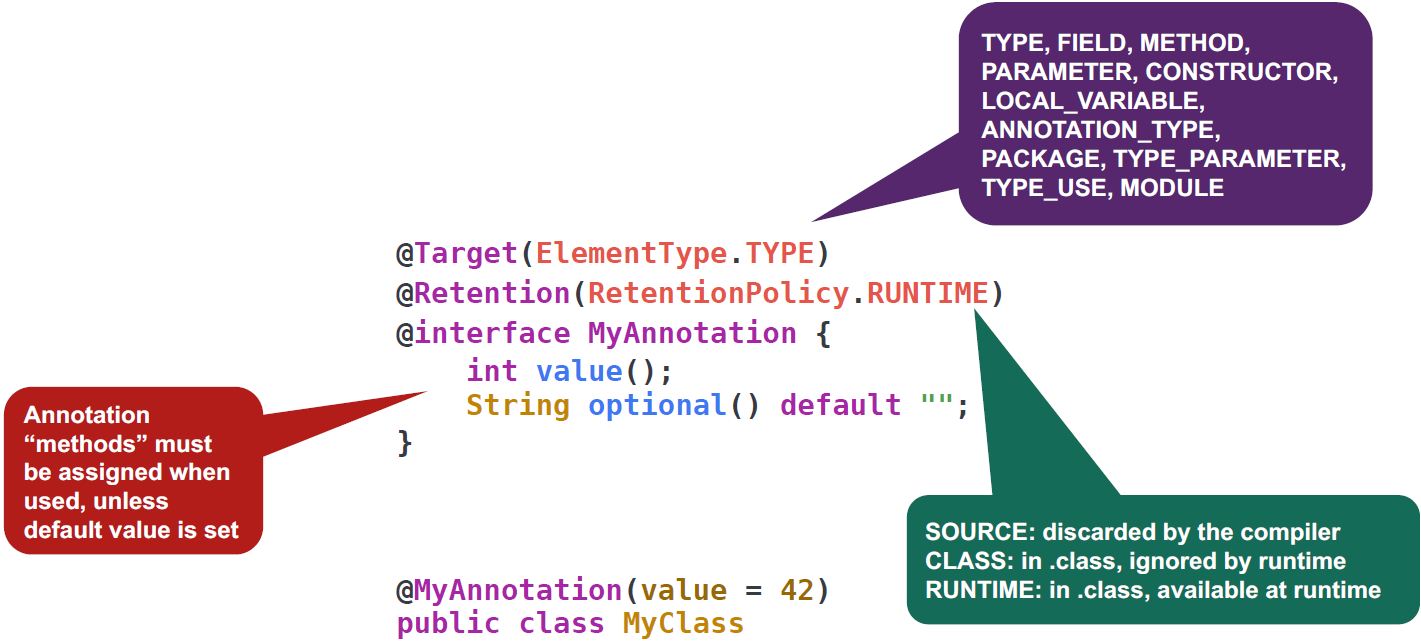
\includegraphics[width=\linewidth]{./img/annotation_declaration.png}
\subsubsection{Processing Annotations}
\begin{itemize}
    \item Depending on retention policy
    \begin{itemize}
        \item processed by compiler
        \item during compilation by Annotation Processors
        \item at runtime using reflection
    \end{itemize}
    \item Processors need to be on the classpath to be recognized by the Java compiler
    \item Compiler then invokes the processor if it finds any annotations the processor has registerd
    \item Processors can generate new files, those can contain additional annotations
\end{itemize}

\subsection{Core Principles}
\begin{itemize}
    \item DI
    \item IoC
    \item Aspect Oriented Programming (AOP)
\end{itemize}

\subsection{Beans}
\begin{itemize}
    \item Form the backbone of the application
    \item Managed by the Spring IoC Container
\end{itemize}
\subsubsection{Scopes}
Control the lifetime of Beans
\begin{itemize}
    \item \textit{singleton}: (default) single object for each Spring IoC Container
    \item \textit{prototype}: Any number of instances
    \item \textit{request}: Lifecycle of a single HTTP request, each has its own instance
    \item \textit{session}: Lifecycle of a HTTP Session
    \item \textit{application}: Lifecycle of a ServletContext 
    \item \textit{websocket}: Lifecycle of a WebSocket
\end{itemize}
\begin{lstlisting}
@Bean 
@Scope('singleton')
public DataSource dataSource() { }
\end{lstlisting}

\subsubsection{Config Simplifications}
\textbf{@Component}: Spring creates beans automatically\\ 
\textbf{@ComponentScan}: Automatic scanning for components\\
\textbf{@Autowired}: Property is mapped to Constructor

\subsubsection{Aspect Oriented Programming (AOP)}
\begin{itemize}
    \item Mitigates cross-cutting concerns
\end{itemize}
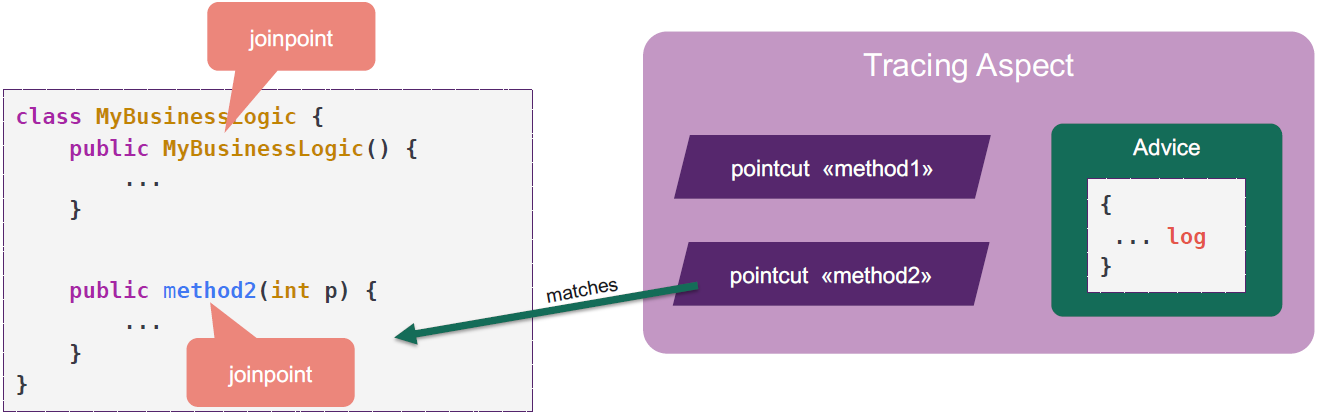
\includegraphics[width=\linewidth]{./img/aop.png}
\begin{itemize}
    \item When a \textit{pointcut} pattern matches a \textit{joinpoint} being executed, an advice can be run
    \item Weaving is the compile or runtime technology to interleave the advice code into the joinpoints
\end{itemize}

\subsubsection{AspectJ}
\begin{itemize}
    \item Technology of Spring AOP
    \item Can be used on all objects
    \item Offers different approaches to weave aspects:
    \begin{itemize}
        \item Compile-time weaving (produces woven class files as output)
        \item Post-Compile weaving (weaves existing class files)
        \item Load-time weaving (binary weaving)
    \end{itemize}
\end{itemize}
        \section{Boxing / Killing}
\subsection{Singleton Boxing / Killing}
\subsubsection{Problem}
\begin{itemize}
    \item Some Classes should have only one instance
    \item The instance must be accessible from a well-known access point 
    \item Subclassing from the Singleton should be possible
    \item Extending the Singleton class must not break existing code
    \item How can be guaranteed that only one oject of a class is instantiated and can globally be accessed?
\end{itemize}
\subsubsection{Solution}
Ensure a class only has one instance and provide a global point of access to it 
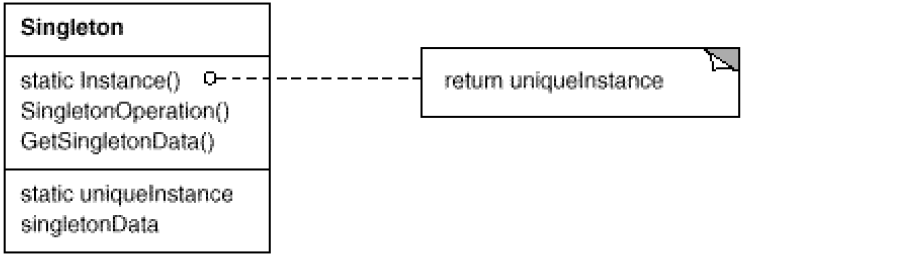
\includegraphics[width=\linewidth]{./img/singleton.png}
\subsubsection{Solutions inside Singleton}
\begin{itemize}
    \item Singleton Pattern
    \item Class Factory Method
    \item Lazy Acquisition
    \item Eager Acquisition
\end{itemize}
\subsubsection{Summary}
\textbf{Benefits}
\begin{itemize}
    \item Controlled access to sole instance
    \item Reduced name space
    \item Permits refinement of operations and representation
    \item Permits variable number of instances
    \item More flexible than class operations
\end{itemize}
\textbf{Liabilities}
\begin{itemize}
    \item Introduces a global variable/state
    \item Prevents polymorphism
    \item Carries state until app closes
    \item Restricts unit testing
\end{itemize}

\subsection{Singleton Variation 'Registry'}
\begin{itemize}
    \item More flexible approach
    \item Uses a registry of singletons
    \item Classes registers their singleton in a well-known registry
\end{itemize}
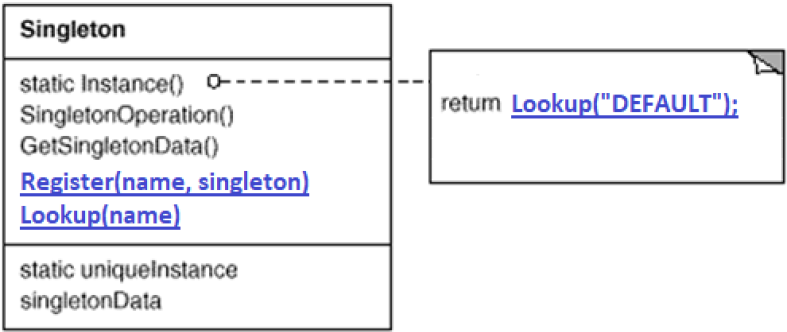
\includegraphics[width=\linewidth]{./img/registry.png}

\subsection{Monostate (Borg) - Killing}
\subsubsection{Problem}
\begin{itemize}
    \item Multiple instances should have the same behaviour
    \item The instances should be simply different names for the same object 
    \item Should have the behaviour of Singleton without imposing the constraint of a single instance
    \item How can two instances behave as though they were a single object?
\end{itemize}
\subsubsection{Solution}
Create a monostate object and implement all member variables as static members 
\begin{lstlisting}
public class Monostate {
    private static int x;
    public int getX() { return x; }
}
\end{lstlisting}
\subsubsection{Summary}
\textbf{Benefits}
\begin{itemize}
    \item Transparency, no need to know about Monostate
    \item Derivability
    \item Polymorphism
    \item Well-defined creation and destruction
\end{itemize}
\textbf{Liabilities}
\begin{itemize}
    \item Breaks inheritance hierarchy
    \item Memory usage
    \item Unable to share Monostate across several tiers
\end{itemize}

\subsection{Service Locator}
\subsubsection{Problem}
\begin{itemize}
    \item Implementation of a global service instance should be exchangeable
    \item It should be possible to execute the service methods on another tier transparently
    \item How could we register and locate global services when one is needed?
\end{itemize}
\subsubsection{Solution}
Implement a service locator that knows how to hold all of the services that an application might need.
\begin{itemize}
    \item Implement the ServiceLocator as a Singleton 'Registry'
    \item ServiceLocator returns \textit{finder} instances, which are used to locate the underlying services
\end{itemize} 
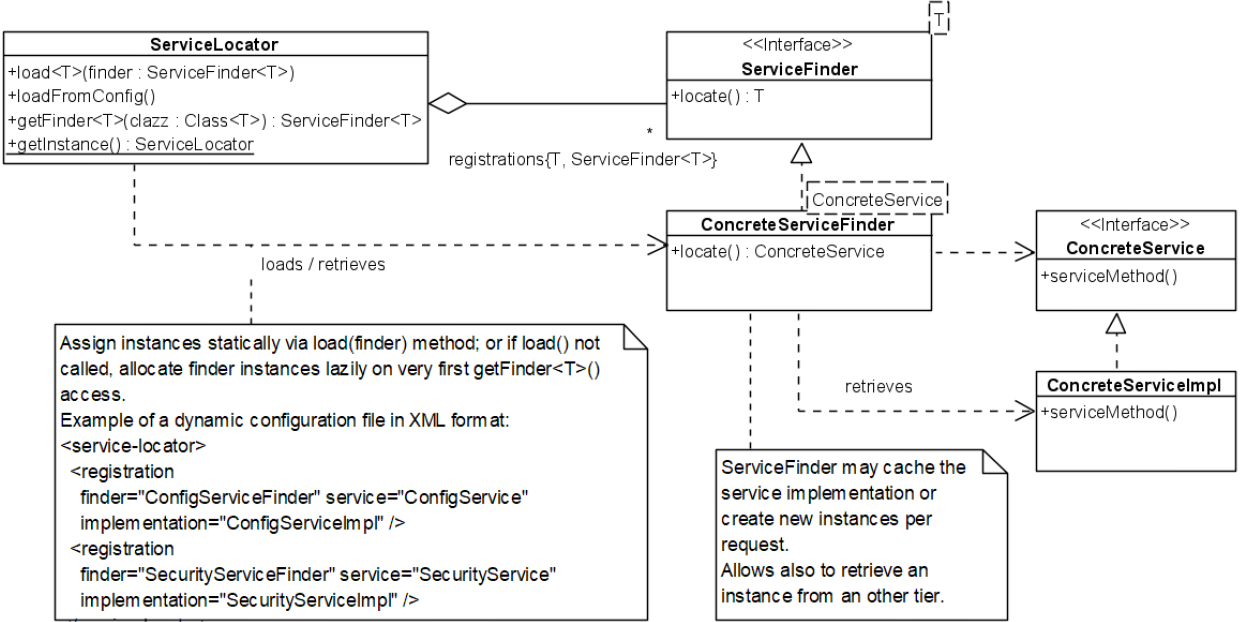
\includegraphics[width=\linewidth]{./img/service_locator.png}
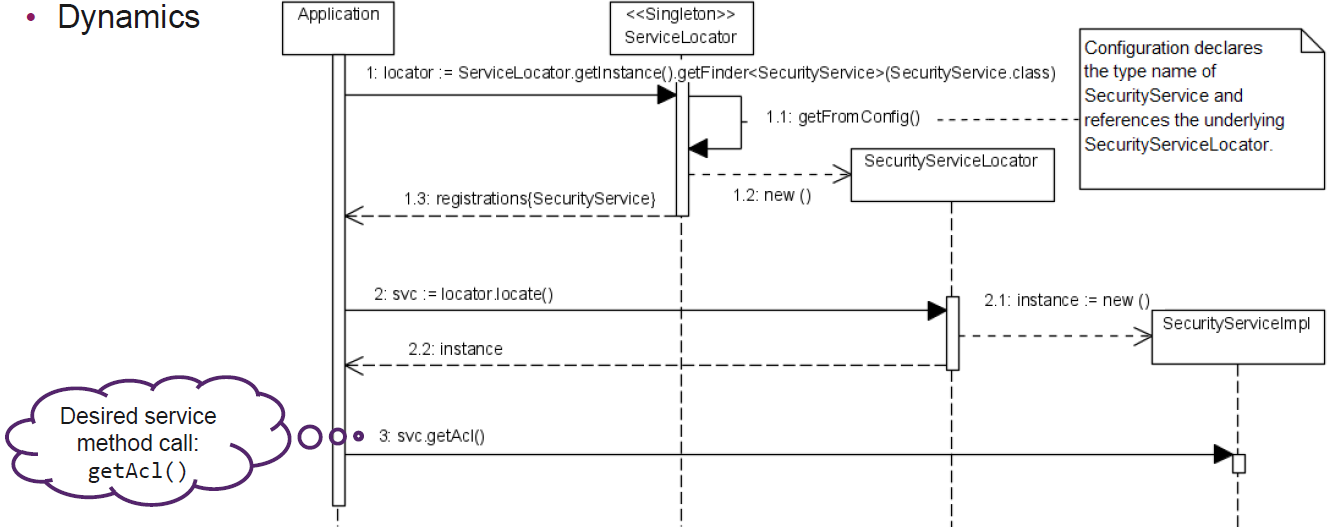
\includegraphics[width=\linewidth]{./img/service_locator_dynamic.png}
\subsubsection{Summary}
\textbf{Benefits}
\begin{itemize}
    \item There is exactly ONE Singleton in the application
    \item ServiceLocator interface strogly rely on abstractness
\end{itemize}
\textbf{Liabilities}
\begin{itemize}
    \item Clients stll rely on a static reference to ServiceLocator class (tight coupling)
    \item No possibility to replace the ServiceLocator 
\end{itemize}

\subsection{Parameterize from Above}
\begin{itemize}
    \item Singleton pattern doesn't provide durability and testability requirements
    \item The application has been layered (horizontally) in a logical manner
    \item How can we povide the required application-wide data to the lower layers without making the data globally accessible?
\end{itemize}
\subsubsection{Solution}
Parameterize each layer from above. Data that affect the behaviour of lower layers should be passed in from the top of the stack.
\begin{itemize}
    \item Pass in configuration parameters and 'known' objects rather than having them global
\end{itemize}
\subsubsection{Summary}
\textbf{Benefits}
\begin{itemize}
    \item No global variables
    \item Implementations of parameterized functionalities are exchangeable
    \item Enforces separation-of-concenrns at architecture level
    \item Reduces coupling between layers
\end{itemize}
\textbf{Liabilities}
\begin{itemize}
    \item Adds more complexity to the system
    \item Contexts must be passed through the whole app stack
    \item Fragile Bootstrapper: app must be wired completely at startup
\end{itemize}

\subsection{Dependency Injection}
\subsubsection{Problem}
\begin{itemize}
    \item User may override implementations of existing app components (e.g. test doubles)
    \item Any Componet within the system can demand an object of a specified interface
    \item The Components should not know anything about the wiring mechanism
\end{itemize}
\subsubsection{Solution}
Introduce a DI Container which loads the interfaces and implementation calsses at startup and dynamically instantiates and wires the objects according to the dependency tree.
\begin{itemize}
    \item Central container
    \item Users reference dependencies by the required interfaces
    \item Users apply code annotations 
    \item Clients should not address the container directly
\end{itemize}
\subsubsection{Implementation}
\begin{itemize}
    \item Combine \textit{Service Locator} and \textit{PfA}
    \item Container class must not be statically referenced by clients
\end{itemize}
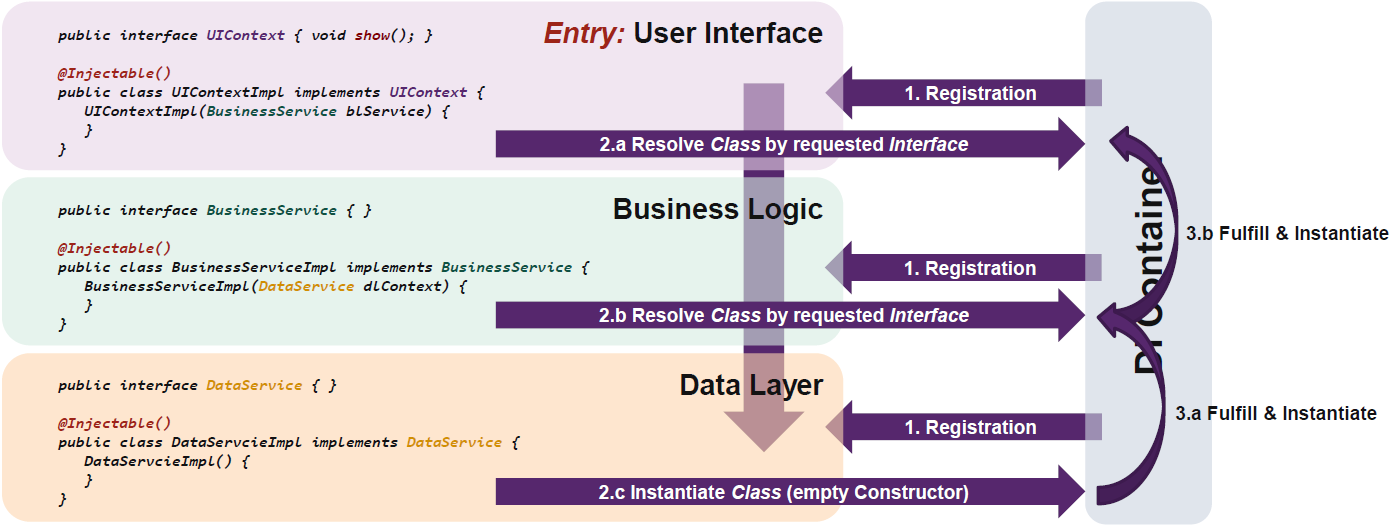
\includegraphics[width=\linewidth]{./img/di_impl.png}
\subsubsection{Summary}
\textbf{Benefits}
\begin{itemize}
    \item Reduces coupling
    \item Contracts between classes are based on interfaces
    \item Suports open/closed principle
    \item Allows flexible replacement of an implementation
\end{itemize}
\textbf{Liabilities}
\begin{itemize}
    \item Adds black magic to the system
    \item Debugging the object dependency tree may become hard
    \item Recursive dependencies are hard to find and may prevent the sytem from startup
    \item Relies on reflection and can result in a performance hit
\end{itemize}
\subsubsection{Discussion}
\textbf{Relation Singleton - DI}
\begin{itemize}
    \item Some injected Dependencies may be singletons
    \item DI Container implementation may be based on 'registry' singleton
\end{itemize}
\textbf{Improvement of DI over Service Locator}
\begin{itemize}
    \item Client classes dont depend directly on the DI Container
    \item Less coupling between DI Container and Component
\end{itemize}

\subsection{Flyweight}
A single pattern for both \textbf{sharing} and \textbf{creation}
\subsubsection{Problem}
\begin{itemize}
    \item Storage costs are high because of the sheer quantity of objects
    \item Many objects bay be replaced by relatively few shared objects
    \item The objects do not depend on object identity
    \item How can multiple copies of a identical constant object be avoided?
\end{itemize}
\subsubsection{Solution}
Use sharing to support large numbers of fine-grained objects efficiently
\begin{itemize}
    \item Flyweight manager maintains instantiated flyweights
    \item Flyweights must be immutable (readonly)
    \item Context information is often maintained by parent object
\end{itemize}
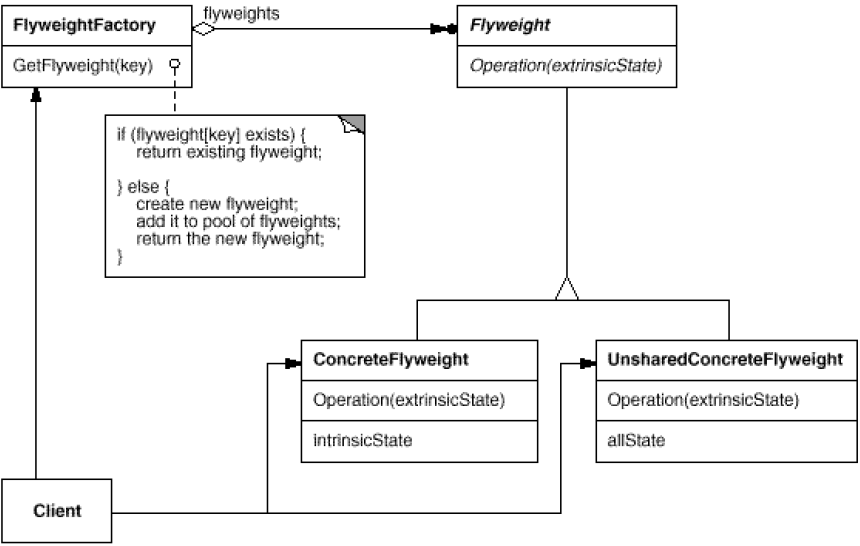
\includegraphics[width=\linewidth]{./img/flyweight.png}
\includegraphics[width=\linewidth]{./img/flyweight_dynamic.png}
\subsubsection{Solutions inside Flyweight}
\begin{itemize}
    \item Composite
    \item Immutable Value
    \item Pooling
    \item Class Factory Method
    \item Lazy Acquisition
    \item Eager Acquisition
\end{itemize}
\subsubsection{Summary}
\textbf{Benefits}
\begin{itemize}
    \item Reduction of the total number of instances (space savings)
\end{itemize}
\textbf{Liabilities}
\begin{itemize}
    \item Can't rely on object identity
    \item May introduce run-time costs
\end{itemize}

\subsection{Pooling (Boxing)}
\subsubsection{Problem}
\begin{itemize}
    \item A fast and predictable access to resources should be provided
    \item Wastage of CPU cycles in repetitious acquisition / release should be avoided
    \item Acquisition / release complexity should be minimized
    \item How can expensive acquisition and release of resources be avoided by recycling resources that are no longer needed?
\end{itemize}
\subsubsection{Solution}
Manage multiple instances of one type of resource in a pool. This pool of resources allows for reuse of released resources.
\begin{itemize}
    \item A resource pool manages resources and gives them to the users
    \item Resource providers, such as OS, owns and manages the resources
\end{itemize}
\includegraphics[width=\linewidth]{./img/pooling.png}
\subsubsection{Implementation}
\begin{itemize}
    \item Define the maximum number of resources that are maintained by the pool
    \item Decide between \textit{eager} and \textit{lazy} Acquisition
    \item Determine resources recycling/eviction semantics
\end{itemize}
\subsubsection{Summary}
\textbf{Benefits}
\begin{itemize}
    \item Performance of app
    \item Simplified release and acquisition of resources
    \item New resources can be created dynamically
\end{itemize}
\textbf{Liabilities}
\begin{itemize}
    \item Certain overhead
    \item Acquisition requests must be synchronized to avoid race conditions
\end{itemize}
\subsubsection{Discussion}
\textbf{Pattern that can be combined with Pooling}
\begin{itemize}
    \item Pool acts as mediator
\end{itemize}
\textbf{Relation of Flyweight and Pooling}
\begin{itemize}
    \item Flyweight implements a pool with immutable resources statically
\end{itemize}
\textbf{Is immutability of named resources key?}
\begin{itemize}
    \item No
\end{itemize}
\textbf{Difference between pooling and caching}
\begin{itemize}
    \item Caching is about handling resources with identity, pooling does not
    \item All resources in a pool are equal
    \item Caching only manages object lifetime in cache, not of objects themselve
\end{itemize}
        \section{Shepherding Process}
\includegraphics[width=\linewidth]{./img/shepherding.png}
\subsection{Process}
\textbf{1. Three Iterations}
\begin{itemize}
    \item How to budget your time and effort to make shepherding effective
\end{itemize}
\textbf{2. The Shepheade Know the Sheep}
\begin{itemize}
    \item How to establish a productive relationship between you and the author
\end{itemize}
\textbf{3. Half a Loaf}
\begin{itemize}
    \item How to make sure that shepheadring continous to move forward
\end{itemize}
\textbf{4. Big Picture}
\begin{itemize}
    \item How to gasp the gist of the pattern right off the bat
\end{itemize}
\textbf{5. Author as Owner}
\begin{itemize}
    \item How to keep from writing the pattern for the author
\end{itemize}
\textbf{6. Forces Define Problem}
\begin{itemize}
    \item How to understand the problem at a deeper level
\end{itemize}

\subsection{Writer's Workshop}
\begin{itemize}
    \item Used to improve patterns
    \item Primary focus of PLoP (PATTERN LANGUAGES OF PROGRAMS)
    \item The authors of the paper under discussion remain silent
    \item Major target: Get a lot of feedback and suggestions
\end{itemize}
\includegraphics[width=\linewidth]{./img/writers_workshop.png}

\subsubsection{1) Pattern Scanning}
Does reading the pattern problem, solution, known uses, context, forces, consequences make sense?

\subsubsection{2) Styling the Forces}
Are forces listed as items?

\subsubsection{3) BUT Style}
\begin{itemize}
    \item Is BUT-Style used and does it build tension?
    \item Does it lead to bold face solution?
\end{itemize}

\subsubsection{4) Detailed Example / Technical Diagram}
Is there a detailed example and technical diagram?

\subsubsection{5) Known Uses}
Are there at least three know and approprate uses

\subsubsection{6) Relationship}
\begin{itemize}
    \item Are the related patterns described in a logical order?
    \item Are the relationships appropriate?
\end{itemize}

\subsubsection{7) Sstand-Alone, Self-Contained}
\begin{itemize}
    \item Does the pattern overlap with other patterns?
    \item Is the pattern description coherent?
    \item Are there suggestions for improvement?
\end{itemize}

    \end{multicols*}
\end{document}























